\documentclass[a4paper,12pt,oneside]{article}

\usepackage{polski}
\usepackage[polish]{babel}
\usepackage[utf8]{inputenc}
\usepackage[T1]{fontenc}  
\usepackage{indentfirst}
\usepackage[pdftex]{graphicx}
\usepackage{pdfpages} 
\usepackage{fancyhdr} %numery stron po zewnętrznej 
\usepackage{wrapfig}
\usepackage{hyperref} 
\usepackage{titlesec} 
\usepackage{color}
\usepackage{xcolor}
\usepackage{listings}
\usepackage[nottoc,numbib]{tocbibind}
\usepackage{multicol}
\usepackage{tabu}
\usepackage{floatrow}

%marginesy 
\usepackage[ bindingoffset = 1cm]{geometry} 
%interlinia 
\linespread{1.2} 

\widowpenalty=10000 % ostatni wierszrkapitu nie zostanie przeniesiony na następną stronę 
\clubpenalty=10000 % pierwszy wiersz akapitu nie będzie kończył strony (nie używam tego ustawienia)
\hbadness= 1450 %% zmniejsza liczę wyświetlanych ostrzeżeń (można zwiększyć, ale bez przesady)
\hfuzz = 0pt %% tekst może sterczeć ma marginesie na 1,5pt (ok. 0,5mm)

\clubpenalty=10000 %nie pozostawia sierot
\brokenpenalty=10000 %nie dzieli stron je»eli podziaª wyrazu
\sloppy %zakaz wydªu»ania lini

%wcięcia 
\setlength{\parindent}{1cm} 
\setcounter{secnumdepth}{2} %only sections and subsections are numbered 
\setcounter{tocdepth}{2} %table of contents shows up to three levels 

\author{Amadeusz Kosik}
\title{Środowisko analizy złośliwego oprogramowania dla systemu Windows}

\lstset{
	basicstyle = \small,
	keywordstyle = \color{black}\bfseries,
	identifierstyle = ,
	commentstyle = \color{white}
	stringstyle = \ttfamily,
	showstringspaces = false
}

\begin{document}
	
	\begin{titlepage} 
	
		\begin{tabu}to \textwidth {c X[c]}
			Politechnika Warszawska & Rok akademicki \\
			Wydział Elektroniki i Technik Informacyjnych& 2015 / 2016 \\
			Instytut Automatyki i Informatyki Stosowanej & 
		\end{tabu}
		
		\begin{center}
		
		\vfill
		
		
\includegraphics[width=5cm]{gfx/logo-pw.jpg}		
		
		\vfill
		
		\Large \textbf{PRACA DYPLOMOWA INŻYNIERSKA} \\[1cm]
		
		\Large Amadeusz Jerzy Kosik \\[1cm] 				
		
		\huge \textbf{System analizy złośliwego~oprogramowania w~systemie~Windows}\\
		
		\vfill
		\vfill
		
		\large
		
		\begin{flushright}
			Opiekun pracy: \\
			dr inż. Piotr Gawkowski
		\end{flushright}
	
		\vfill
		
		% Bottom of the page
		\large{Warszawa, 2016 r.}
		
		\end{center}
	
	\end{titlepage} 
	\pagestyle{empty}
	\cleardoublepage 	
	
	\renewcommand\abstractname{STRESZCZENIE}
	\begin{abstract}	
		Praca prezentuje autorski system MESS (ang. \textit{Malware Evaluation Support System}), wspomagający analizę dynamiczną złośliwego oprogramowania poprzez częściowe zautomatyzowanie procesu uruchamiania i~obserwacji badanego programu. System składa się z~odpowiednio skonfigurowanych maszyn wirtualnych, na których jest uruchamiane analizowane oprogramowanie, serwera zarządzającego ich pracą oraz prostych skryptów klienckich służących do komunikacji pomiędzy poszczególnymi komponentami systemu oraz użytkownikiem.
		
		System MESS dostarcza informacji o~wykonywanych przez badaną aplikację działaniach w~systemie Windows oraz~o~jej komunikacji z~innymi komputerami za pośrednictwem Internetu. Wraz z systemem MESS skonfigurowano zestaw narzędzi monitorujących, ale jednocześnie użytkownik ma możliwość łatwego dodania kolejnych narzędzi. 
	
		\vfill

		Słowa kluczowe: bezpieczeństwo, wirtualizacja, złośliwe oprogramowanie
	\end{abstract}		
	\hrulefill
		
	\renewcommand\abstractname{ABSTRACT}
	\begin{abstract}
		\begin{center}		
			{\bfseries Windows-based Malware analysis system} \\[0.3cm]
		\end{center}
			
		This thesis describes the MESS (Malware Evaluation Support System) which is designed to automatize the process of running and observing malware application. It consists of a set of virtual machines prepared to safely run malware applications on them, a server which manages the virtual machines and client applications written as console scripts responsible for communication between user and the system.
		
		The MESS gathers information about activities performed by the malware under the analysis in the Windows system and its network communication over the Internet. Although the system is equiped with a set of monitoring tools, additional ones can be easily provided to be used in a sample evaluation process. 

		\vfill	

		Keywords: malware, security, virtualization 
	\end{abstract}	
	
	\newpage	
	\thispagestyle{empty}
	\cleardoublepage 
		
	\newpage
	\tableofcontents
	\newpage
	
	\pagestyle{plain}
	\pagenumbering{arabic}
	
	\section{Wstęp}
	Wstęp do niniejszej pracy zawiera krótki opis tematyki złośliwego oprogramowania, którego praca dotyczy oraz cel i uzasadnienie tworzenia środowiska analizy. Następnie przedstawiona jest budowa pracy razem z~krótkim opisem zawartości kolejnych rozdziałów.
	
	\subsection{Charakterystyka złośliwego oprogramowania}	
	\textit{Złośliwe oprogramowanie} (ang. \textit{malware}), będące przedmiotem zainteresowania tejże pracy, jest określeniem aplikacji mających na celu zapewnienie korzyści (w tym także finansowych) twórcy aplikacji bądź zaszkodzenie osobom trzecim. Jego działania (infekcję) można podzielić na trzy fazy \cite{qnap-malware, www-malware-phases}. Pomimo, iż nie wszystkie fazy są wspólne dla każdego rodzaju istniejącego złośliwego oprogramowania, obrazują one dobrze wymagania i~trudności związane z~projektowaniem środowiska kontrolowanego ich uruchamiania i~obserwacji.
	
	\subsubsection{Rozpoznanie}
	
	Jest to zawsze pierwsza faza ataku. Ma ona na celu znalezienie sposobu, w~który złośliwe oprogramowanie zostanie przesłanie i~uruchomione na~komputerze ofiary. Cel ten można osiągnąć na wiele sposobów. Najczęściej wykorzystuje się w~tym celu odpowiednio przygotowane witryny internetowe, wyposażone w~wykorzystujące istniejące luki w~przeglądarkach skrypty JavaScript bądź kontrolki Flash (tzw. \textit{exploit}). Gdy ofiara odwiedza taką stronę, na jej komputer ściągana i~uruchamiana jest złośliwa aplikacja. 
	
	Inną metodą umieszczenia złośliwego na maszynie ofiary jest wykorzystanie inżynierii społecznej, aby użytkownik sam uruchomił udostępniony mu program. W~tym celu atakujący najczęściej wysyłają pocztą elektroniczną podrobione dokumenty takie, jak faktury \cite{www-niebezp-kaspersky} lub powiadomienia z~banku (bądź innych instytucji finansowych). Popularne jest również wysyłanie wiadomości mających wzbudzić ciekawość odbiorcy i~w~ten sposób zachęcić go do odwiedzenia strony lub otworzenia załącznika \cite{www-niebezp-fb}.
	
	\subsubsection{Pobranie i uruchomienie}
	
	Kolejną fazą przebiegu infekcji jest pobranie i~uruchomienie złośliwej aplikacji. Ze względu na popularność oprogramowania antywirusowego, coraz częściej zamiast "pełnego" programu najpierw pobierany jest tzw. \textit{downloader}, czyli prosty program mający na celu pobranie i~rozpakowanie właściwej aplikacji. Ponieważ nie wykonuje on żadnych podejrzanych z~punktu widzenia oprogramowania antywirusowego działań, nie jest zazwyczaj wykrywany przez działającą na maszynie ofiary ochronę rezydentną programu antywirusowego.
	
	Niektóre ze złośliwych programów po uruchomieniu wykonują dodatkowe czynności, by jak najbardziej utrudnić ich skuteczne wykrycie bądź usunięcie. Przykładami takich działań jest modyfikacja bądź usuwanie plików zainstalowanego oprogramowania antywirusowego i~zapory sieciowej, filtrowanie ruchu sieciowego w~celu uniemożliwienia pobrania narzędzi mogących go wykryć i~usunąć, jak również wyłączanie niektórych usług lub funkcjonalności systemu Windows (np. zablokowanie możliwości uruchomienia systemu w~trybie awaryjnym lub wyłączenie usługi Windows Update \cite{www-virus-winupdate}).
	
	\subsubsection{Działanie docelowe}	
	
	W ostatnim etapem infekcji złośliwe oprogramowanie jest już zainstalowane i~uruchomione na komputerze ofiary. Może więc ono przejść do swojego właściwego zadania (normalnej pracy), zdefiniowanego przez jego autora. W wielu przypadkach oznacza jest to osiągnięcie korzyści przez jego autora bądź przez osobę zlecającej stworzenie tegoż programu. Obecnie najczęstszym jest to:
	
	\begin{itemize}
		\item \emph{Kradzież danych dostępowych użytkownika}, np. numerów kart płatniczych, loginów i haseł do serwisów internetowych. 
		\item \emph{Kradzież plików osobistych}, np. zdjęć, dokumentów. Skradzione dane są potem wykorzystywane do szantażu ofiary bądź też udostępniane publiczne.
		\item \emph{Tworzenie sieci zdalnie kontrolowanych komputerów} (ang. \textit{botnet}).
	\end{itemize}
	
	Powyższa lista nie wyczerpuje wszystkich istniejących przypadków. Oprócz złośliwego oprogramowania mającego na celu zainfekowanie jak największej liczby maszyn, tworzone są również aplikacje przeznaczone do zaatakowania bardzo precyzyjnie określonego celu, jak np. robak Stuxnet \cite{www-stuxnet}.
	
	Wspomnieć należy również, iż w ramach swojej normalnej pracy złośliwe oprogramowanie często podejmuje działania mające na celu propagację siebie pomiędzy na inne maszyny. Dotyczy to w~szczególności aplikacji rozprzestrzeniających się pomiędzy stacjami roboczymi, np. za pomocą poczty elektronicznej lub komunikatorów, za pomocą których wysyłane są przez złośliwy program wiadomości do osób zapisanych w~kontaktach tychże programów.
	
	\subsection{Podział złośliwego oprogramowania}
	
	Ze względu na duże zróżnicowanie zarówno celu, jak i~sposobu jego osiągania przez złośliwe oprogramowanie, można dokonać jego podziału na następujące kategorie:
	
	\subsubsection{Exploit} 
	Exploit jest prostym programem wykorzystującym znane przez jego autora podatności w~systemie Windows lub zainstalowanym oprogramowaniu. Jest on ajczęściej wykorzystywany do rozpoczęcia infekcji (poprzez pobranie i uruchomienie właściwej części złośliwego programu). Może nim być np. skrypt JavaScript, applet Java, kontrolka ActiveX bądź Flash, odpowiednio spreparowany plik \textit{.doc} lub \textit{.pdf}. Ze względu na regularne wydawanie aktualizacji przez twórców przeglądarek, większość programów tego typu jest użytecznych tylko przez pewien krótki czas.
	
	\subsubsection{Ransomware}
	Złośliwe oprogramowanie tego typu wykorzystywane jest do osiąganie korzyści materialnych poprzez szantaż. Po uruchomieniu program tego typu pobiera ze zdalnego serwera klucz szyfrujący, który następnie jest użyty do~zaszyfrowania wszystkich plików użytkownika. Kolejnym krokiem jest poinformowanie użytkownika o~tym oraz wyświetlenie instrukcji, w~jaki sposób ofiara może odzyskać swoje pliki. Wiąże się to najczęściej z~wpłatą środków na konto szantażysty (zazwyczaj w~walucie wirtualnej, np. Bitcoin).
		
	\subsubsection{Rootkit}	
	Jest to program mający na celu ukrycie siebie oraz wybranych innych programów przed systemem operacyjnym i~innymi aplikacjami. Zazwyczaj jest wykorzystywany razem z~złośliwym programem innego typu.
				
	\subsubsection{Worm}
	Robak (ang. \textit{Worm}) to złośliwy program rozprzestrzeniający się automatycznie bez zgody i~wiedzy użytkownika. W~tym celu najczęściej wykorzystywana jest poczta elektroniczna, komunikatory internetowe bądź sieć P2P. Oprócz samopowielania, robak wykonuje także typowe operacje dla złośliwego oprogramowania (p. podrozdział 1.1, \textit{Działanie docelowe}). \\				
				
	Ze względu na zagrożenie jakie niesie ze sobą złośliwe oprogramowanie, bardzo istotnym zadaniem jest przeciwdziałanie rozprzestrzenianiu się tegoż. W~tym celu stosuje się narzędzia takie jak \textit{zapory sieciowe} czy \textit{oprogramowanie antywirusowe}. Nie mogą one działać nie znając potencjalnego zagrożenia, czyli samego złośliwego oprogramowania. Nie zapewniają tym samym bezpieczeństwa przed tzw. zagrożeniem dnia zerowego (ang. \textit{zero-day vulnerability}), dlatego bardzo ważne jest również skuteczne identyfikowanie i~analizowanie nowych zagrożeń. Ciągły rozwój złośliwego oprogramowania niesie ze sobą konieczność rozwijania metodyki analizowania go.
			
	\subsection{Sposoby analizy złośliwego oprogramowania}	
	Analizę oprogramowania (nie tylko złośliwego) przeprowadzić można na dwa sposoby: statycznie -- poprzez analizę zdeasemblowanego (bądź zdekompilowanego) kodu aplikacji, bądź dynamiczne -- uruchamiając próbkę w specjalnie przygotowanym w tym celu środowisku i obserwując zmiany zachodzące w nim. Sposoby te, ze względu na odmienność podejścia nie wykluczają się wzajemnie i nie stanowią dla siebie zamienników. Stosować je można równocześnie. W dalszej części pracy program (z~założenia złośliwy) poddany analizie nazywany jest \textit{próbką}.
	
	\subsubsection{Analiza statyczna}	
	Analiza statyczna polega na zdeasemblowaniu bądź zdekompilowaniu kodu posiadanej aplikacji i określeniu na jego podstawie działania programu. Choć zazwyczaj jest to efektywne podejście, w przypadku złośliwego oprogramowania może okazać się bardzo trudne bądź niemożliwe. W celu oszukania skanerów antywirusowych i utrudnienia analizy statycznej autorzy złośliwego oprogramowania stosują techniki zaciemniające kod tworzonych przez nich programów, uniemożliwiając efektywną analizę \cite{book-malware, for-dynamic-anal, for-antivm-antidbg}. Do takich technik należą np. modyfikacja kodu w trakcie działania aplikacji (np. poprzez wykorzystanie szyfrowania XOR lub ROT13 do zaszyfrowania części kodu bądż wstawienie fałszywych instrukcji zamienianych po uruchomieniu na instrukcje NOP),
	bądź też wywoływanie instrukcji powrotu z funkcji do funkcji bez wywołanej instrukcji wejścia.
	
	\subsubsection{Analiza dynamiczna}		
	W odróżnieniu od analizy statycznej, w ramach analizy dynamicznej zakładany jest niejako model badanej próbki jako \textit{czarnej skrzynki}, której zachowanie w systemie jest monitorowane. Analiza wymaga przeprowadzenia eksperymentu - uruchomienia próbki w odpowiednim środowisku, gdzie uruchomione są programy monitorujące zasoby i sam system \cite{for-dynamic-anal}. Wyniki (logi) działania tychże programów są następnie wykorzystywane do zbadania, jakie czynności w systemie wykonuje badana próbka.
	
	Dla złośliwego oprogramowania przeznaczonego dla systemu operacyjnego (jak w~niniejszej pracy) środowiskiem wykonywania jest cały system operacyjny. Ze względów praktycznych korzystne jest zastosowanie maszyn wirtualnych. Pozwala to na jednoczesne uruchomienie wielu analiz na jednej fizycznej maszynie oraz zapewnia proste przygotowywanie i~czyszczenie środowiska pomiędzy kolejnymi analizami poprzez mechanizm migawek maszyn wirtualnych (ang. \textit{snapshot}). Wiąże się to jednak również z ryzykiem wykrycia przez próbkę, że działa ona na maszynie wirtualnej. Sposobów na wykonanie takiego sprawdzenia jest wiele \cite{for-antivm-antidbg}. Najprostsze z nich ograniczają się do sprawdzenia, czy na dysku znajdują się ślady użytkowania systemu przez człowieka, takie jak zmieniona tapeta pulpitu czy zawartość zapisana w~pamięci podręcznej przeglądarki. Bardziej wyrafinowanymi metodami jest natomiast sprawdzenie w~rejestrze systemu danych procesora i~porównanie np. liczby wątków zgłoszonych w~systemie operacyjnych z~liczbą podawaną przez producenta procesora.
			
	Konstruując środowisko uruchomieniowe dla złośliwego oprogramowania należy przede wszystkim mieć na uwadze kwestie bezpieczeństwa. Organizację eksperymentów komplikuje fakt, że odcięcie środowiska od świata zewnętrznego (sieci Internet) uniemożliwiłoby przeprowadzenie pełnej analizy, ponieważ złośliwe oprogramowanie często do działania wymaga do niego dostępu. Część aplikacji złośliwych jest rozprzestrzeniana w~formie programu inicjującego atak, którego zadaniem po uruchomieniu jest ściągnięcie i wykonanie właściwej jego części. Egzemplarze należące do kategorii botnetu wymagają łączności z~serwerem zarządzającym w~celu pobierania z~niego rozkazów do wykonania na zarażonej maszynie. Badana próbka nie może mieć jednak dostępu do innych maszyn w sieci lokalnej ani do gospodarza maszyn wirtualnych (w przypadku gdy środowisko uruchomieniowe jest maszyną wirtualną). Sam dostęp do Internetu powinien być zatem filtrowany i monitorowany. Badana próbka nie powinna mieć też możliwości łączenia się po portach takich, jak np. \textit{25, 587} (wykorzystywanych przez złośliwe oprogramowanie do masowego wysyłania spamu).
			
	Do zagadnienia analizy dynamicznej można podejść na dwa sposoby: monitorując próbkę w trakcie jej działania (\textit{online}) lub porównując stan środowiska, w~którym się wykonywała, ze stanem sprzed uruchomienia próbki. Podobnie jak w przypadku podziału analizy na statyczną i dynamiczną, obie metody nie wykluczają, ale wzajemnie się uzupełniają.
	
	\subsubsection{Analiza porównawcza}	
	Jednym ze sposobów analizy działania badanej próbki jest porównanie stanu systemu sprzed oraz po jej uruchomieniu. Obiektem zainteresowania są zmiany wykryte w~środowisku (np. w systemie plików lub w rejestrze systemu). Główną zaletą takiej analizy jest bardzo niski stopień ingerencji w badaną próbkę i~jej otoczenie. Analizowany program nie jest w stanie wykryć działania narzędzi wykorzystywanych w trakcie analizy porównawczej. Dzięki temu ryzyko, że analiza nie powiedzie się jest niskie. Do wad natomiast należy z całą pewnością mała ilość informacji o przebiegu działania badanej próbki. Wynikiem takiej analizy jest jedynie pewien stan systemu. Jedną z najbardziej istotnych informacji traconych przy analizie polegającej wyłącznie na analizie porównawczej są logi ruchu sieciowego.
	
	\subsubsection{Monitorowanie uruchomienia z zewnątrz}	
	Monitorowanie środowiska uruchomieniowego próbki z~innej maszyny (wirtualnej bądź fizycznej) jest kolejnym sposobem prowadzenia analizy. W~odróżnieniu od analizy porównawczej, podejście to pozwala na zbieranie informacji o~działaniu analizowanej próbki. Jednocześnie wyeliminowane jest ryzyko, że badana próbka wykryje, iż jest monitorowana. Należy jednakże zwrócić uwagę, iż z~poziomu innej maszyny monitorować można jedynie wybrane zasoby, np. ruch sieciowy. Niemożliwe jest obserwowanie stanu systemu operacyjnego (w~tym również uruchomionych w~nim programów i~ich wątków) bez ingerowania bezpośrednio w system, na którym próbka została uruchomiona.
	
	\subsubsection{Monitorowanie procesu w środowisku uruchomieniowym}	
	Trzecim sposobem przeprowadzenia analizy dynamicznej próbki jest monitorowanie uruchomionego jej procesu w czasie rzeczywistym przy użyciu narzędzi zainstalowanych na tej samej maszynie (w tym samym systemie operacyjnym). Podejście to dostarcza najbardziej szczegółowych informacji nt. działania próbki i~jej interakcji z innymi procesami i~systemem operacyjnym. Należy jednakże zauważyć, iż taka forma analizy dynamicznej wiąże się z~ryzykiem wykrycia przez próbkę narzędzi monitorujących, a~więc również i~z~niepowodzeniem wykonania analizy. Szczególnie narażone na ryzyko niepowodzenia jest wykorzystanie do analizy debuggera - ingeruje on w~systemowy proces obserwowanej aplikacji w~znacznie większym stopniu, niż narzędzia stricte monitorujące, przez co jego wykrycie jest zdecydowanie łatwiejsze \cite{book-malware,for-ultimate-antidbg,for-antivm-antidbg}.
			
	\subsection{Cel pracy}	
	Wykonane w ramach niniejszej pracy system MESS (ang. \textit{Malware Evaluation Support System} - system wsparcia ewaluacji złośliwego oprogramowania) jest środowiskiem dynamicznego monitorowania w~czasie rzeczywistym badanej próbki złośliwego oprogramowania. Jego zadaniem jest przeprowadzanie eksperymentów - automatyczne uruchamienie dostarczonej przez użytkownika próbki złośliwego oprogramowania w środowisku wyposażonym w~programy monitorujące w czasie rzeczywistym takie parametry jak stan systemu operacyjnego, ruch sieciowy, uruchomione aplikacje i~ich wątki, czy też istotne operacje systemowe (m.in. na systemie plików bądź rejestrze systemowym). Po zatrzymaniu eksperymentu użytkownik otrzymuje raport zawierający informacje zgromadzone przez owe narzędzia. Zakres monitorowania (i co za tym idzie, szczegółowość uzyskiwanych wyników analizy), zależy wyłącznie od funkcjonalności i~konfiguracji wykorzystywanych narzędzi monitorujących. W przeprowadzonych w~ramach tej pracy eksperymentach wykorzystano narzędzia ProcessMonitor (monitor systemu Windows) oraz Wireshark (monitor ruchu sieciowego).
	
	Oprócz automatyzacji procesu analizy, zadaniem środowiska jest również zapewnienie odpowiedniego poziomu bezpieczeństwa wykonywanych analiz. Badane oprogramowanie powinno mieć odpowiednio ograniczony dostęp do sieci Internet oraz być odizolowane od użytkownika oraz sieci lokalnej.
			
	\subsection{Układ pracy}
	Niniejsza praca składa się z~siedmiu rozdziałów. W~rozdziale drugim znajduje się opis istniejących rozwiązań z~zakresu wspomagania analizy złośliwego oprogramowania. Rozdział trzeci przedstawia wymagania, które zostały postawione na etapie projektowania systemu MESS. Czwarty rozdział traktuje o~szczegółach architektury i implementacji środowiska. W piątym rozdziale przedstawiony jest opis wykorzystania środowiska w~celu zbadania próbki oprogramowania. Ostatni rozdział zawiera podsumowanie pracy i~potencjalne możliwości rozbudowy środowiska.
			
	\newpage
			
	\section{Przegląd istniejących rozwiązań}
	
	Istnieją dostępne, gotowe rozwiązania pozwalające na wykonanie analizy dynamicznej próbki złośliwego oprogramowania. Poniższy rozdział zawiera krótki opis wybranych systemów.
	
	\subsection{Anubis}
	
	Anubis \cite{www-anubis} jest udostępnioną przez International Secure Systems Lab, bezpłatną dla zastosowań niekomercyjnych usługą analizy programów niewymagających zainstalowania przed użyciem, w tym również złośliwych. Użytkownik może za jej pomocą wykonać analizę dynamiczną pliku binarnego dla systemu Windows lub Android. Aplikacje stworzone dla pierwszego z~nich uruchamiane są w~systemie Windows~XP. Ponieważ Anubis jest rozwiązaniem o~zamkniętych źródłach, nie są dostępne informacje o~jego implementacji ani wykorzystywanych przez niego platformach wirtualizacji.
	
	Aby wykonać analizę przy użyciu Anubisa, użytkownik musi posiadaną próbkę wysłać za pomocą formularza na stronie WWW, poczty email lub przy użyciu dostarczanego skryptu w~języku Python. Próbki przesyłane przez użytkowników są umieszczane w~kolejce (p. rysunek \ref{gfx-anubis-queue}). W~momencie, gdy analizy wszystkich poprzednich aplikacji zostaną zakończone uruchamiana jest analiza próbki użytkownika. Trwa ona do momentu zakończenia uruchomionego przez usługę procesu dostarczonej aplikacji lub do przekroczenia czasu oczekiwania (określanego jako \textit{timeout}), którego znaczenie nie zostało niestety wyjaśnione przez twórców.
	
	\begin{figure}[ht]
		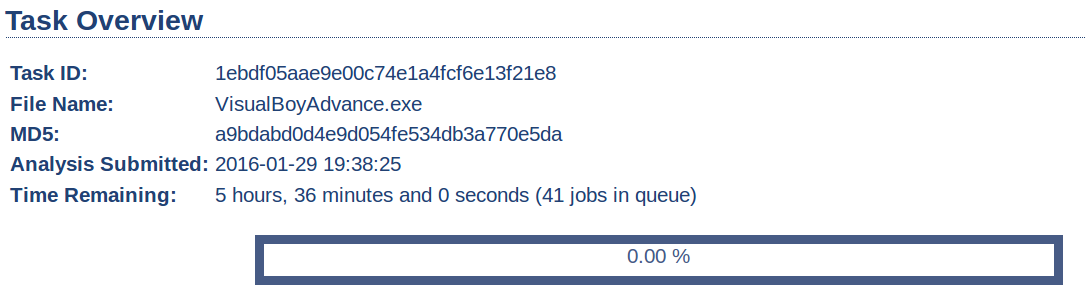
\includegraphics[scale=0.35]{gfx/anubis-queue.png}
		\caption{Ekran próbki oczekującej na analizę w~kolejce Anubisa}
		\label{gfx-anubis-queue}
	\end{figure}
	
	Po zakończeniu analizy użytkownikowi dostarczany jest raport z~działania w~systemie próbki i~jej procesów potomnych. Składa się on z części tekstowej oraz ewentualnie załączników takich jak plik zrzutu ruchu sieciowego (w~formacie \textit{.pcap}). Raport tekstowy zawiera krótkie podsumowanie, w~którym wymienione są rodzaje wykrytych aktywności z~ich oceną szkodliwości dla systemu ofiary (rysunek \ref{gfx-anubis-report}) oraz części właściwej, w~której opisane są zaobserwowane aktywności uruchomionej próbki oraz utworzonych przez nią wątków. Należą do nich m.in.:	
	\begin{itemize}
		\item lista utworzonych bądź zmodyfikowanych plików,
		\item operacje na rejestrze systemowym,
		\item utworzone procesy i wątki,
		\item wczytane biblioteki DLL,
		\item ruch sieciowy zainicjowany przez aplikację.
	\end{itemize}
	
	\begin{figure}[ht]
		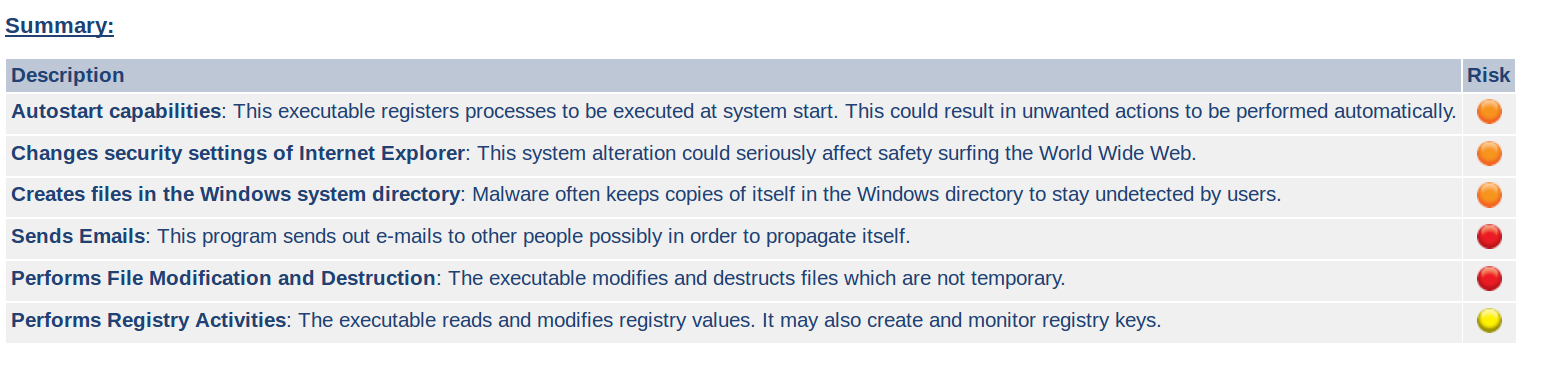
\includegraphics[scale=0.26]{gfx/anubis-report.png}
		\caption{Podsumowanie w~przykładowym raporcie Anubisa}
		\label{gfx-anubis-report}
	\end{figure}
	
	Do wad Anubisa z~pewnością należy fakt, iż jest on udostępniany jedynie w~formie usługi. W~czasie pisania tejże pracy średni czas oczekiwania na uruchomienie analizy podesłanej próbki wynosił około jednej godziny, co dyskwalifikuje Anubisa w~wykorzystaniu przy automatycznej analizie ilościowej złośliwego oprogramowania. Ponadto, generowane przez usługę raporty pozwalają określić działanie próbki w~bardzo ogólnym zakresie. Dane o~zdarzeniach w~systemie operacyjnym (np. utworzeniu wątku) są mocno przefiltrowane. W~przypadku wykrycia modyfikacji pliku nie jest użytkownikowi podawana zawartość pliku po tejże operacji (rysunek \ref{gfx-anubis-filemod}). Wspomnieć należy również o~niedoskonałości generowanych przez Anubisa podsumowań - np. wysłany do analizy program nienależący do złośliwego oprogramowania został sklasyfikowany jako potencjalnie szkodliwy, ponieważ po uruchomieniu utworzył swój plik konfiguracyjny (\textit{Performs File Modification and Destruction}).
	
	\begin{figure}[ht]
		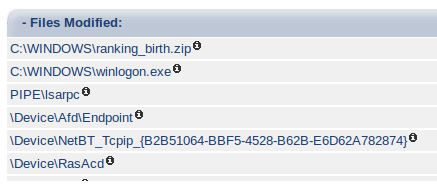
\includegraphics[scale=0.6]{gfx/anubis-file-mod.png}
		\caption{Wykryta przez Anubis modyfikacja pliku}
		\label{gfx-anubis-filemod}
	\end{figure}
	
	\subsection{Capture-HPC}
	
	Capture-HPC \cite{www-hpc} jest systemem przeznaczonym do wyszukiwania stron internetowych zawierających kod infekujący maszynę klienta. Przeprowadzenie eksperymentu przy użyciu tegoż narzędzia polega na dostarczeniu adresów stron internetowych, które \textit{Capture-HPC} odwiedza przy użyciu różnego rodzaju aplikacji klienckich (popularne przeglądarki WWW, pakiety biurowe, odtwarzacze multimediów itp.). W przypadku, gdy odwiedzana witryna zawiera złośliwy kod (tzw. exploit), a wykorzystywana aplikacja kliencka posiada odpowiednie dla niego luki (podatności), dochodzi do (kontrolowanej) infekcji systemu operacyjnego. Kolejnym krokiem analizy jest sprawdzenie przez Capture-HPC, czy doszło do niepożądanych zmian w~systemie (takich jak zmiany w~rejestrze systemowym bądź modyfikacja plików znajdujących się na dysku). 
	
	Eksperymenty wykonywane w~środowisku \textit{Capture-HPC} wykonywane są wewnątrz dedykowanych maszyn wirtualnych pracujących na platformie VMWare. System pozwala na użycie zarówno lokalnej platformy wirtualizacji, jak i~wykorzystanie maszyn zainstalowanych na innych maszynach fizycznych, co~pozwala na znacznie lepszą skalowalność poziomą całego systemu. 
	
	Na całe środowisko Capture-HPC, oprócz maszyn wirtualnych, składa się również serwer zarządzający. Jest on odpowiedzialny za komunikację z~użytkownikiem oraz przekazywanie maszynom wirtualnym adresów stron do przeanalizowania.
	
	Istotną wadą rozwiązania jest jego brak aktywnego rozwoju i~utrzymania - ostatnie zmiany w~projekcie pochodzą z roku 2008. Na~stronie projektu znajduje się wiele nierozwiązanych zgłoszeń o~błędach, w~tym także krytycznych. Ponadto, oficjalnie wspierana wersja VMWare Server to 1.0, podczas gdy w~chwili pisania tejże pracy aktualną wersją stabilną jest 2.0.
	
	\subsection{Maltester}
	
	Maltester \cite{weiti-maltester} jest środowiskiem analizy dynamicznej utworzonym w~ramach pracowni dyplomowej na Wydziale Elektroniki i Technik Informacyjnych Politechniki Warszawskiej. Służy on do przeprowadzania analizy porównawczej stanu maszyny przed i~po uruchomieniu badanej próbki.
	
	Podobnie jak wymienione wyżej środowiska analizy, Maltester pracuje w~oparciu o~platformę wirtualizacji, a~dokładniej - platformę Xen. Eksperyment przeprowadzany jest na maszynie pracującej pod kontrolą systemu Windows XP, na którym nie ma zainstalowanych jakichkolwiek narzędzi monitorujących. W~trakcie działania próbki monitorowany jest tylko ruch sieciowy pomiędzy maszyną a~siecią Internet. Po zatrzymaniu maszyny wirtualnej badane są zmiany w pamięci operacyjnej oraz na dysku twardym maszyny wirtualnej. Do tego celu służą moduły analityczne aplikacji. 
	
	W~odróżnieniu do środowiska opisywanego w niniejszej pracy, celem Maltestera jest dostarczenie informacji o~skutkach działania próbki w~systemie operacyjnym, a nie jego przebieg. Innymi słowy środowisko MESS nie zastępuje funkcjonalnie Maltestera, ale go uzupełnia.
	
	\subsection{Podsumowanie}
	
	Ze względu na bardzo dynamiczny rozwój złośliwego oprogramowania, istotna jest możliwość szybkiej adaptacji systemu, przy użyciu którego jest ono analizowane. Warunek ten jest spełniony wyłącznie poprzez rozwiązania otwartoźródłowe, dlatego istnieje potrzeba tworzenia własnych rozwiązań w~środowisku akademickim. Ponadto, system analizy powinien umożliwiać pracę z~różnymi wirtualizatorami i~narzędziami monitorującymi oraz~pozwalać na łatwe dostosowanie do ich nowych wersji. Z~kolei z~punktu widzenia docelowego użytkownika systemu analizy, tworzenie przez środowisko raportów w~formie tekstowej nie jest istotne. Znacznie większe znaczenie ma ilość i~jakość danych otrzymanych po~przeprowadzeniu eksperymentu. System powinien więc udostępniać wszystkie zarejestrowane zdarzenia, a filtrowanie i dalsza obróbka powinna się odbywać pod kontrolą użytkownika. 
	
	Powyższe obserwacje zostały uwzględnione przy projektowaniu systemu MESS. Jego kod źródłowy jest dostępny dla pracowników instytutu, a~architektura tegoż systemu - modularna, dzięki czemu można w~prosty sposób zmodyfikować system i~dostosować go do obsługi scenariuszy nieprzewidzych podczas etapu projektowania. Możliwe jest również łatwe dostosowanie systemu do pracy z~platformą wirtualną inną niż wykorzystana w~ramach tejże pracy oraz praca z~wieloma wirtualizatorami jednocześnie. System nie tworzy raportów ani analiz na podstawie eksperymentów, a~ich wyniki dostarczane są w~formie surowej. Choć zawęża to krąg potencjalnych użytkowników systemu do osób dobrze obeznanych z~problematyką złośliwego oprogramowania, to jednocześnie pozwala to na wydobycie większej ilości informacji na podstawie jednego eksperymentu.
	
	\clearpage
	\newpage
	
	\section{Analiza wymagań}	

	Poniższy rozdział prezentuje oczekiwania wobec wykonanego systemu. Rozdział otwiera opis typowego scenariusza użycia tegoż systemu, po czym sformułowane są wymagania funkcjonalne i niefunkcjonalne.
		
	\subsection{Scenariusz użycia}
	
	Zadaniem systemu MESS jest uruchamianie próbek złośliwego oprogramowania w~kontrolowanym, obserwowanym systemie Windows na maszynie wirtualnej. Typowy przypadek użycia systemu w~celu przeprowadzenia analizy aplikacji wygląda następująco:
	
	\subsubsection{Przygotowanie środowiska}
	
	Pierwszym krokiem jest przygotowanie środowiska do uruchomienia dostarczonej przez użytkownika próbki na odpowiednio do tego celu przygotowanej maszynie wirtualnej (zainstalowane odpowiednie oprogramowanie użytkowe - w~tym wersje z~podatnościami, pożądane aktualizacje systemu operacyjnego, uruchomione określone usługi i~aplikacje symulujące istnienie użytkownika końcowego itp.). Maszyna taka znajdować się powinna w stanie gotowym do odebrania i~uruchomienia próbki - i~w~takim stanie zapamiętana w~migawce maszyny wirtualnej. Użytkownik dostarcza systemowi MESS nazwę maszyny wirtualnej, na której eksperyment ma zostać uruchomiony, nazwę pliku próbki pod jaką zostanie ona zapisana na maszynie wirtualnej oraz sam plik próbki. Ma on również możliwość przekazania zestawu narzędzi i~skryptów przewidzianych do uruchomienia w~razie wystąpienia:
	\begin{itemize}
		\item rozpoczęcia analizy: skrypt wykonywany jest przed uruchomieniem próbki,
		\item restartu systemu operacyjnego maszyny wirtualnej, na której próbka jest uruchomiona: skrypt wykonywany jest przed wymuszeniem ponownego uruchomienia systemu operacyjnego,
		\item zakończenia analizy: skrypt jest wykonywany przed przygotowaniem i~pobraniem wyników eksperymentu.
	\end{itemize}
	Wszystkie w/w skrypty wykonywane są na maszynie wirtualnej, na której uruchomiona została próbka.
		
	Po otrzymaniu żądania użytkownika i~sprawdzeniu jego kompletności sprawdzany jest stan wybranej do wykonania analizy maszyny wirtualnej. Rozpoczynanie eksperymentu na pracującej maszynie (tj. takiej, na której jest już uruchomiony inna jest próbka) jest zabronione.
	
	Jeżeli natomiast wskazana maszyna jest dostępna, system wczytuje jej zapisany stan i~uruchamia ją. Następnie informacje niezbędne do rozpoczęcia eksperymentu są przekazywane na maszynę wirtualną. Na tejże maszynie uruchamiane są narzędzia monitorujące (zarówno wbudowane, jak i~dostarczone przez użytkownika). Kolejnym krokiem jest uruchomienie dostarczonej próbki złośliwego oprogramowania. Po utworzeniu w~systemie operacyjnym procesu próbki maszyna wirtualna jest oznaczana jako będąca w użyciu, a~użytkownik otrzymuje informację zwrotną o~rezultacie rozpoczęcia eksperymentu. 
	
	\subsubsection{Monitorowanie działającej aplikacji}
	
	W~czasie trwania eksperymentu ze strony użytkownika nie jest wymagana żadna interakcja z systemem MESS.	Może on natomiast zażądać restartu maszyny wirtualnej oraz podejrzeć ruch sieciowy pomiędzy maszyną a siecią. 
	
	Możliwość wykonania restartu systemu operacyjnego maszyny wirtualnej wynika ze specyfiki działania złośliwych aplikacji. Niektóre z~nich po uruchomieniu jedynie instalują się w~systemie operacyjnym ofiary. Docelowe działanie takiego programu ma miejsce dopiero po ponownym uruchomieniu systemu. 
	
	Wykonanie restartu składa się z~dwóch kroków. Najpierw, jeżeli istnieje, wywoływany jest dostarczony przez użytkownika skrypt. Następnie wymuszany jest restart systemu operacyjnego. Po ponownym uruchomieniu maszyny wirtualnej narzędzia monitorujące są uruchamiane, by zachować ciągłość obserwacji. 
		
	\subsubsection{Zatrzymanie obserwacji i~zebranie wyników}
	
	Zakończenie eksperymentu jest wykonywane wyłącznie na życzenie użytkownika. Po  otrzymaniu przez system MESS żądania, na maszynie wirtualnej zatrzymywane są narzędzia monitorujące próbkę, po czym wykonywane są odpowiednie skrypty przesłane przez użytkownika. Rezultat jest następnie udostępniany do pobrania systemowi MESS w formie archiwum ZIP. System pobiera z~maszyny wirtualnej udostępniony plik i~wysyła go użytkownikowi. Na zakończenie fazy system MESS zamyka maszynę wirtualną, przywraca jej zapisany stan i~oznacza ją jako niebędącą w użyciu.
	
	Po zatrzymaniu obserwacji system jest gotowy do uruchomienia kolejnego eksperymentu na poprzednio użytej maszynie wirtualnej.
	
	\subsubsection{Natychmiastowe zatrzymanie obserwacji}
	
	Oprócz standardowego zakończenia eksperymentu z~pobraniem wyników, użytkownik ma możliwość natychmiastowego zakończenia (przerwania) eksperymentu. W~przypadku takiego żądania nie jest wykonywana przez system faza tworzenia i~pobierania pliku archiwum z wynikami, następuje jedynie zatrzymanie i~odtworzenie stanu maszyny wirtualnej. Podobnie jak w przypadku zatrzymania z~pobraniem wyników, po zatrzymaniu natychmiastowym użyta maszyna wirtualna znów jest gotowa do wykonania kolejnego eksperymentu.
	
	Zatrzymanie natychmiastowe jest przewidziane do obsługi sytuacji, gdy:
	\begin{itemize}
		\item badana próbka wyłączyła na maszynie wirtualnej aplikację odpowiedzialną za komunikację z~systemem MESS, uniemożliwiając zatrzymanie eksperymentu z~pobraniem wyników;
		\item użytkownik zaobserwował, iż uruchomione złośliwe oprogramowanie wykonuje niepożądane czynności w~sieci, np. uczestniczy w~ataku DDOS lub~próbuje dokonać włamania na serwer należący do osób trzecich,
		\item użytkownik zdecydował, że nie jest już dłużej zainteresowany wynikami uruchomionego eksperymentu.
	\end{itemize}
		
	\subsection{Monitorowanie próbki i~format wyników}
	
	Bardzo istotną kwestią z punktu widzenia użytkownika systemu MESS jest dobór narzędzi monitorujących działającą próbkę. Określa on, jakie dane będą wynikiem eksperymentu oraz jaki będzie ich poziom szczegółowości. Na potrzeby analizy złośliwego oprogramowania dla systemu Windows największe znaczenie mają dwie kategorie aktywności: ruch sieciowy pomiędzy Internetem a~zainfekowaną maszyną oraz zdarzenia systemowe mające miejsce na tejże maszynie. Potrzeby te są zaadresowane poprzez wbudowane w system MESS narzędzia:
	
	\subsubsection{Process Monitor}
	
	Process Monitor \cite{tool-procmon} jest narzędziem służącym do monitorowania zdarzeń systemowych w~systemie Windows. Jak jego nazwa wskazuje, służy on do obserwacji aktywności uruchomionych w~systemie procesów. Pozwala on na obserwację zdarzeń takich, jak:
	\begin{itemize}
		\item operacje na rejestrze systemowym (odczyt i zapis wartości bądź kluczy),
		\item operacje na plikach (utworzenie, modyfikacja, usunięcie),
		\item tworzenie i zatrzymywanie wątków bądź procesów aplikacji.
	\end{itemize}
	
	Każde zaobserwowane przez Process Monitor zdarzenie zawiera informacje takie, jak nazwa i ścieżka procesu wywołującego je oraz jego rezultat. Niektóre zdarzenia mają także informacje o~ich czasie trwania bądź też stosie wywołań.
	
	Aplikacja umożliwia zapisywanie zebranych we~wskazanym przez użytkownika pliku, jak również na uruchomienie w~tle (bez okna GUI). Plik wynikowy może mieć format CSV, XML bądź natywny PML. Aplikacja pozwala również na zdefiniowanie filtrów, które będą użyte w~czasie działania aplikacji.
	
	\subsubsection{Wireshark}
	
	Wireshark \cite{tool-wireshark} jest pakietem służącym do analizy ruchu sieciowego. Zawiera on narzędzia pozwalające na monitorowanie ruchu sieciowego, jego pogląd w~czasie rzeczywistym oraz odczytywanie uprzednio zapisanych plików w formacie \textit{.pcap}.
	
	Na potrzeby zautomatyzowanego prowadzenia eksperymentów wykorzystane zostało narzędzie \textit{dumpcap}. Jego przeznaczeniem jest monitorowanie ruchu sieciowego na danym interfejsie sieciowym. Po uruchomieniu narzędzie zapisuje przechwycone pakiety w~pliku logu w formacie \textit{.pcap}.
	
	\subsection{Format wyników}
	
	Utworzone przez powyższe aplikacje pliki są po zakończeniu eksperymentu przekazywane użytkownikowi w postaci archiwum ZIP jako rezultat eksperymentu. Ze względu na możliwość dodawania przez użytkownika dowolnych narzędzi i~skryptów, zawartość archiwum nie ma ściśle określonej struktury. 
	
	Możliwość wykonania restartu systemu operacyjnego maszyny, na której prowadzony jest eksperyment, powoduje, iż zebrane pliki wynikowe działania narzędzi wbudowanych są grupowane w~katalogach. Katalogi te mają nazwy odpowiadające dacie i godzinie uruchomienia wbudowanych w~system MESS narzędzi (na skutek rozpoczęcia analizy bądź restartu systemu operacyjnego). Pozwala to użytkownikowi na zorientowanie się w~kolejności utworzenia tychże plików.
				
	\subsection{Wymagania funkcjonalne}
	\begin{itemize}
		\item Eksperymenty powinny być prowadzane na maszynie wirtualnej działającej pod kontrolą systemu Windows, który powinien mieć dostęp do sieci Internet.
		\item System powinien pozwalać na uruchamianie i zatrzymywanie analizy z~maszyn zdalnych za pomocą stosownego oprogramowania klienckiego.
		\item Użytkownik powinien mieć możliwość zażądania restartu maszyny wirtualnej, po wykonaniu którego pracę powinny wznowić narzędzia monitorujące.
		\item Użytkownik powinien mieć możliwość wyboru narzędzi, które zostaną użyte do monitorowania próbki w czasie eksperymentu:
		\begin{itemize}
			\item system powinien umożliwiać wybór, które z narzędzi zainstalowanych w~systemie operacyjnym maszyny wirtualnej mają być uruchomione w~czasie eksperymentu,
			\item system powinien umożliwiać użytkownikowi dołączanie dodatkowych narzędzi i skryptów na czas pojedynczego eksperymentu. Dostarczane skrypty powinny być uruchamiane odpowiednio podczas rozpoczęcia, zakończenia analizy i~restartu systemu operacyjnego maszyny wirtualnej.
		\end{itemize}
		\item Użytkownik powinien mieć możliwość podglądu ruchu sieciowego pomiędzy maszyną wirtualną a siecią zewnętrzną.	
		\item Na żądanie użytkownika aplikacja dostarcza wyniki działania wszystkich narzędzi monitorujących uruchomionych podczas eksperymentu.
		\item Jeżeli pozwalają na to zasoby sprzętowe, system powinien umożliwiać prowadzenie równoległe eksperymentów na wielu maszynach wirtualnych. Eksperymenty te powinny być od siebie niezależne (tj. zatrzymanie jednej analizy nie może wpływać na pozostałe, będące w toku).
	\end{itemize}
	
	\subsection{Wymagania niefunkcjonalne}
	\begin{itemize}
		\item System powinien mieć budowę modularną, aby w przyszłości możliwa była wymiana wykorzystywanej platformy wirtualizacji lub wbudowanie nowych narzędzi monitorujących.
		\item System powinien mieć możliwość pracy z maszynami wirtualnymi znajdującymi się na więcej niż jednym serwerze wirtualizacji.
		\item Maszyna wirtualna nie może mieć dostępu do sieci lokalnej, w~której pracuje system MESS, natomiast dostęp do sieci Internet maszyny wirtualnej musi być do pewnego stopnia ograniczony. Uruchamiana w~ramach eksperymentu próbka nie może wykonywać określonych działań szkodliwych, np. wysyłać spamu. Ze względów bezpieczeństwa filtr ruchu sieciowego musi być założony poza maszyną wirtualną.
	\end{itemize}
			
	\clearpage
	\newpage
	
	\section{Projekt rozwiązania}
			
	W poniższym rozdziale znajduje się projekt systemu MESS, to jest jego ogólna architektura oraz oczekiwane scenariusze działania i~ich rezultat. Opisane zostały również napotkane trudności implementacyjne oraz potencjalne problemy w~skutecznym użytkowaniu narzędzia.
			
	\subsection{Architektura rozwiązania}
	
	System MESS jest zaprojektowany i~przeznaczony do działania na wielu maszynach fizycznych bądź wirtualnych. Jego standardowa konfiguracja obejmuje następujące maszyny: Kontroler, Nadzorcę oraz Wykonawców. Konfiguracja ta jest przedstawiona na rysunku~\ref{gfx--schema-basic-logical}.
	
	\begin{figure}[h!]
		\includegraphics[scale=0.25]{gfx/schema-arch-basic.png}
		\caption{Standardowa konfiguracja systemu MESS - podział logiczny}
		\label{gfx--schema-basic-logical}
	\end{figure}			
	
	Kontroler jest główną częścią systemu. Odpowiada on za sterowanie pozostałymi maszynami oraz~za~komunikację z~użytkownikiem. Jako jedyny nie może być powielony w~ramach jednego działającego systemu, ale może być zarówno maszyną fizyczną, jak i wirtualną. 
	
	Wykonawcą jest maszyna wirtualna, na której uruchamiane są obserwowane próbki złośliwego oprogramowania.
	
	Nadzorcą nazywana jest maszyna, na której zainstalowana została platforma wirtualizacji goszcząca maszyny wirtualne Wykonawców. Odpowiada ona za~wykonywanie operacji na Wykonawcach, tj. uruchamianie, zatrzymywanie i~przywracanie stanu z~migawki. Możliwe jest skonfigurowanie środowiska tak, aby obsługiwanych było wielu Nadzorców. Ze względu na wymagania sprzętowe dostępnych platform wirtualizacji, każdy Nadzorca musi być maszyną fizyczną -- w~maszynach wirtualnych nie są dostępne technologie Intel-VT/AMD-V, których wymagają współczesne wirtualizatory.

	\subsubsection{Skalowanie systemu MESS}
		
	System MESS został zaprojektowany tak, by możliwe było jego skalowanie poziome. W~tym celu system obsługuje zarówno wielu Wykonawców, jak również i~Nadzorców. Ponadto Kontroler systemu MESS może być przeniesiony na odrębną maszynę fizyczną. Konfiguracja taka jest przedstawiona na rysunku \ref{gfx--schema-arch-advanced}.	
	
	\begin{figure}[h!]
		\includegraphics[scale=0.25]{gfx/schema-arch-advanced.png}
		\caption{Rozproszona konfiguracja systemu MESS}
		\label{gfx--schema-arch-advanced}
	\end{figure}
	
	System MESS nie wymaga, by wszyscy Nadzorcy udostępniali taką samą platformę wirtualizacji. Z tego względu możliwe jest wykorzystanie skalowalności systemu w~celu częściowego obejścia problemu wykrywania poszczególnych typów wirtualizacji przez badane próbki poprzez jednoczesne zastosowanie różnych wirtualizatorów. Takie rozwiązanie pozwala użytkownikowi systemu określić, które z~dostępnych mu rozwiązań wirtualizacji jest wykrywane przez badany program, a~które pozwalają na wykonanie analizy.	
		
	\subsection{Platforma wirtualizacji}
	Jak wspomniano wcześniej, projektowany system wykorzystuje maszyny wirtualne, na których będą przeprowadzane eksperymenty. Aby możliwe było zautomatyzowanie procesu prowadzenia eksperymentów, wirtualizacje wykorzystywane przez system platformy powinny pozwalać na wykonywanie poniższych operacji:
	\begin{itemize}
		\item sprawdzanie stanu maszyny wirtualnej (tj. czy maszyna pracuje, czy jest wyłączona),
		\item uruchamianie i zatrzymywanie maszyny,
		\item zapisywanie i wczytywanie z pliku stanu maszyny (migawki / punktu kontrolnego)
	\end{itemize}
	
	Powyższe operacje muszą być możliwe do wywołania za pomocą programistycznego API bądź komendy lub programu w linii poleceń lub skryptu.
				
	Ze względu na powyższe wymagania wybrano platformę \textit{Hyper-V} \cite{www-hyperv}. Jest ona dostępna dla systemów Windows w wersji od 8 (oraz Windows Server 2008) wzwyż. Jej zaletą jest API, za pomocą którego możliwe jest wykonywanie wszelkich dostępnych operacji na platformie i jej maszynach wirtualnych - zarówno z poziomu aplikacji, jak i skryptów \textit{PowerShell}. Nie oznacza to jednak, iż pozostałe platformy są z~systemem MESS niekompatybilne.
				
	\subsection{Dostarczanie przez użytkownika narzędzi}
	
	Narzędzia monitorujące użytkownika powinny być dostarczone w formacie archiwum ZIP i zawierać przynajmniej jeden skrypt z~podanych poniżej:
	\begin{itemize}
		\item \textit{before.ps1} - skrypt PowerShell, który jest uruchamiany przed uruchomieniem próbki,
		\item \textit{restart.ps1} - skrypt PowerShell, który jest uruchamiany przed restartem maszyny Wykonawcy,
		\item \textit{after.ps1} - skrypt PowerShell, który jest uruchamiany przed pobraniem wyników eksperymentu.
	\end{itemize}
	Poza wymienionymi plikami, w~dostarczonym archiwum mogą znajdować się inne pliki, w~szczególności mogą być to inne aplikacje lub skrypty wywoływane przez powyższe skrypty.
	
	\subsection{Potencjalne problemy}
	Z przeprowadzaniem obserwacji próbek złośliwego oprogramowania wiążą się pewne problemy. Największą trudność stanowi dobranie zbioru danych wynikowych tak, by z~jednej strony zawierał wszystkie istotne dla użytkownika informacje, a~jednocześnie jak najmniejszą ilość danych niepotrzebnych (np. ruchu sieciowego spowodowanego aktualizowaniem się systemu operacyjnego w~tle). W~przypadku niektórych programów monitorujących możliwe jest zastosowanie filtrowania interesujących użytkownika obserwacji. Pozwala to istotnie zmniejszyć rozmiar danych uzyskanych z eksperymentu, ale istnieje też ryzyko, że wśród odfiltrowanych obserwacji znaleźć się mogą również te związane z działaniami obserwowanej próbki. Problem ten można również w~pewnym stopniu ograniczyć odpowiednio konfigurując system na maszynie wirtualnej. Działania takie jak wyłączenie automatycznego sprawdzania aktualizacji systemu i zainstalowanych programów może istotnie zredukować niepożądane obserwacje narzędzi monitorujących. Problem ten został również napotkany w~czasie testów systemu, gdy podczas każdego uruchamiania analizy, działający w~tle program aktualizujący przeglądarkę internetową pobierał jej nową wersję (ok. 40MiB), zaśmiecając pliki logów narzędzi monitorujących dużą ilością bezużytecznej informacji.
	
	Z~kwestią aktualizacji oprogramowania zainstalowanego na~Wykonawcach wiąże się również zagadnienie właściwego przygotowania samego Wykonawcy. Wykorzystywanie na potrzeby wykonywania analiz nieaktualnych wersji oprogramowania nie daje aktualnego obrazu sytuacji, przez co jej celowość jest dosyć ograniczona. Wykorzystywanie natomiast jedynie najnowszych wersji uniemożliwia szczegółowe porównywanie działania dwóch (lub więcej) próbek -- takowe porównanie wymaga zapewnienia identycznych warunków działania badanego programu. Optymalnym rozwiązaniem jest przechowywanie różnych wersji stanu Wykonawcy (np. przed i~po aktualizacji systemu bądź programów takich, jak przeglądarka internetowa). W~systemie MESS jest to możliwe dzięki wykorzystywaniu różnych migawek stanu Wykonawcy.
	
	Równie istotnym problemem jest wrażliwość próbek na konfigurację środowiska uruchomieniowego. Próbka taka może się nie wykonać w środowisku MESS, (np. z~powodu braku zainstalowanej w~systemie operacyjnym Wykonawcy aplikacji niezbędnej do działania próbki \cite{for-antivm-antidbg}), a~związany z nią eksperyment będzie bezużyteczny. 
		
	Kolejną istotną przeszkodą w wykonywaniu eksperymentów może być wykrycie przez próbkę, iż działa ona na maszynie wirtualnej. Taki program po wykryciu platformy zakończy swoje działanie, nie wykonując właściwej (szkodliwej) części kodu. W czasie pracy z~systemem MESS napotkano kilka próbek, które wykrywały pracę wirtualizatora -- jedna z takich aplikacji wykryła działanie Hyper-V. Inna próbka, która wykrywała działające środowisko Xen systemu Maltester, wykonała sekwencję instrukcji sugerujących sprawdzanie obecności wirtualizacji, ale nie wykryła środowiska Hyper-V, co świadczy o~komplementarności obu systemów.
			
	\newpage	
	
	\section{Implementacja}
	Niniejszy rozdział zawiera opis implementacji systemu MESS. We wstępie znajduje się prezentacja szczegółów architektury systemu oraz jego modułów. W dalszej części umieszczone są definicje zastosowanych API i spodziewany format plików wynikowych eksperymentu. Następnie przedstawione są szczegóły implementacji systemu wraz z uzasadnieniem podjętych decyzji projektowych.	
	
	\subsection{Architektura systemu}		
	
	\begin{figure}[ht]
		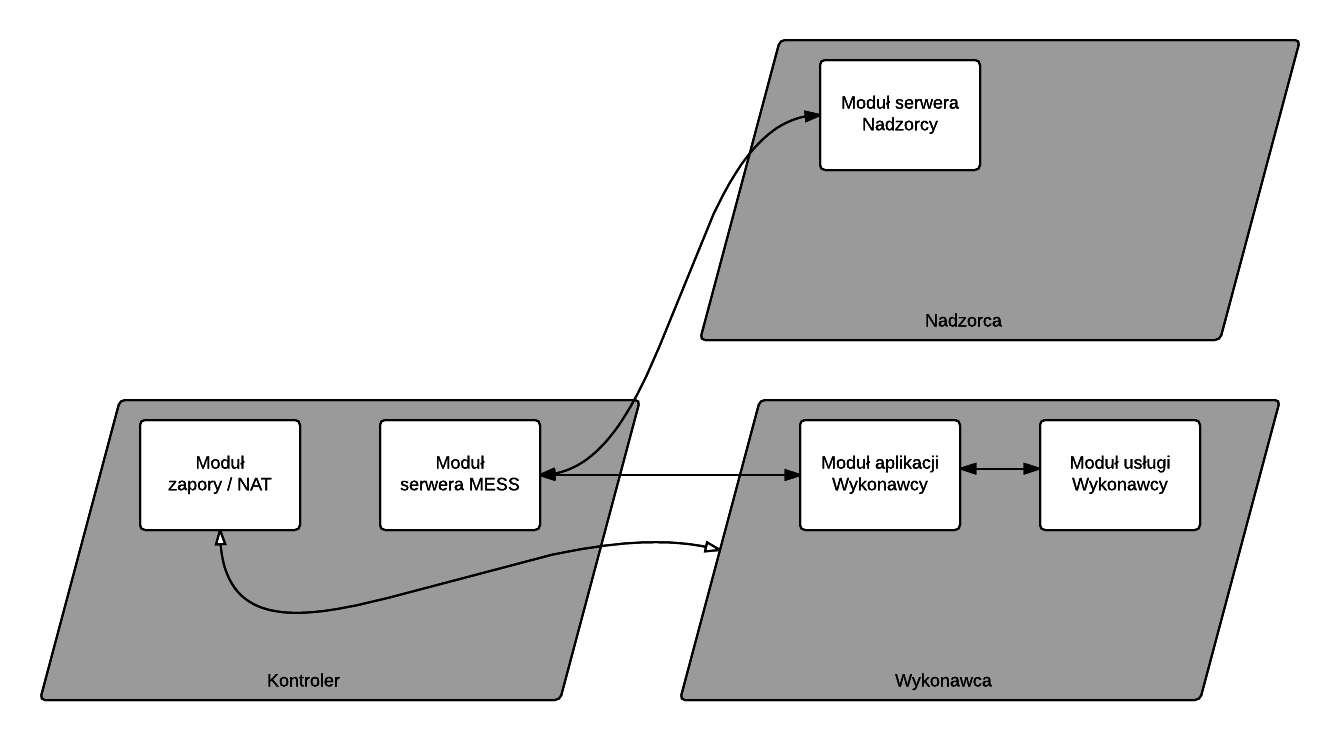
\includegraphics[scale=0.7]{gfx/schema-architecture.png}
		\caption{Schemat architektury systemu}
	\end{figure}	
	
	System MESS ma budowę modularną, gdzie każdy z modułów ma ściśle określone zadanie w ramach całego systemu. Ponadto moduły są rozdzielone pomiędzy trzy typy maszyn obecnych w systemie. Te maszyny to:
	\begin{itemize}
		\item \textbf{Kontroler}
		
		Jest on główną maszyną systemu MESS. Odpowiada on za komunikację z użytkownikiem, Nadzorcą i Wykonawcami. Wykonuje on również całą logikę operacji dostępnych w systemie oraz filtrowanie ruchu sieciowego pomiędzy Wykonawcami a Internetem. W jego skład wchodzą następujące moduły:
		
		\begin{itemize}			
			\item \textbf{Moduł serwera MESS}
			
			Moduł serwera MESS jest głównym modułem systemu. Jest on odpowiedzialny za komunikację pomiędzy użytkownikiem a~systemem MESS oraz za wykonywanie zażądanych operacji.
			W ramach modułu uruchamiany jest osobny wątek serwera XMLRPC. Przez cały czas działania aplikacji nasłuchuje on poleceń użytkownika i~obsługuje je.
						
			\item \textbf{Moduł zapory sieciowej / NAT}
			
			Moduł ten odpowiada za filtrowanie oraz udostępnianie połączenia sieciowego Wykonawcom. Moduł ten również blokuje możliwość nawiązywania połączeń z maszyn Wykonawców do wszelkich adresów znajdujących się w sieci lokalnej. Nie rejestruje on natomiast ruchu sieciowego -- odbywa się to na maszynie Wykonawcy.
			
		\end{itemize}
		
		Poza wymienionymi powyżej modułami, na maszynie Kontrolera znajduje się też serwer HTTP, poprzez który udostępniane są klientowi archiwa z wynikami ostatnich eksperymentów. Ze względu na ograniczoną pojemność dysku przetrzymywanych jest ostatnich 10 wyników (liczba ta jest konfigurowalna), a starsze pliki są usuwane. Ponadto użytkownik ma możliwość zażądania wykonania usunięcia wszystkich poza żądaną liczbą ostatnich archiwów.

		Kontroler może pracować zarówno na maszynie fizycznej, jak i~wirtualnej; w niektórych przypadkach jedna maszyna może być jednocześnie Kontrolerem i Nadzorcą. Jednakże w wybranej przeze mnie implementacji wykorzystującej platformę Hyper-V nie ma możliwości zainstalowania tejże platformy na systemie z rodziny Linux, dlatego kontrolerem jest odrębna maszyna wirtualna. MESS posiada wbudowane zabezpieczenia przed wykorzystaniem maszyny Kontrolera (jak również maszyn nie należących do środowiska) do uruchamiania próbek.
		
		\item \textbf{Nadzorca maszyn wirtualnych}
		
		Nadzorcą maszyn wirtualnych jest maszyna, na której zainstalowana jest platforma wirtualizacji. Jego rolą jest obsługa maszyn wirtualnych Wykonawców, tj. ich uruchamianie, zatrzymywanie oraz przywracanie. Do poprawnego działania wymagane jest połączenie sieciowe pomiędzy Kontrolerem a Nadzorcą. W ramach systemu MESS Nadzorca zawiera tylko jeden moduł:
		
		\begin{itemize}
			\item \textbf{Moduł serwera Nadzorcy}
			
			Moduł serwera Nadzorcy jest odpowiedzialny za odbieranie komunikatów od Kontrolera i~wykonywanie na ich podstawie odpowiednich operacji na maszynach wirtualnych Wykonawców. Nie zawiera on żadnej logiki sterującej systemu; stanowi on adapter pomiędzy systemem MESS a~interfejsem platformy wirtualizacyjnej. 
			
			Moduł nadzorcy jest wyposażony we wbudowane zabezpieczenie sprawdzające nazwę maszyny, dla której żąda się zmiany stanu. Na maszynach innych niż Wykonawcy nie są przeprowadzane żadne operacje, a~w~odpowiedzi na takie żądania wysyłany jest komunikat o~błędzie.
		\end{itemize}
		
		Ze względu na ograniczenia funkcjonalne dostępnych platform wirtualizacji Nadzorca musi być maszyną fizyczną. System operacyjny zainstalowany na maszynie Nadzorcy jest określony przez wybraną platformę wirtualizacji. Dla niniejszej implementacji jest to Windows Server 2012 R2.
		
		\item \textbf{Wykonawca}
		
		Wykonawca jest maszyną, na której przeprowadzane są eksperymenty. Musi on być umieszczony na maszynie wirtualnej kontrolowanej przez Nadzorcę. W~przeciwieństwie do Kontrolera i Nadzorcy, Wykonawca jest uruchomiony tylko na czas trwania eksperymentu. Ze względów bezpieczeństwa nie może on również inicjować połączeń z innymi maszynami systemu MESS -- może jedynie odbierać połączenia.
		
		Wszystkie maszyny wirtualne Wykonawców muszą mieć nazwy rozpoczynające się od \textit{MW} (\textit{MESS Worker}). Wymaganie to wynika z~konieczności prostej identyfikacji przez Nadzorcę roli maszyny w~środowisku - nie powinien on umożliwiać operowania na stanie maszyn innych niż Wykonawcy.
		
		Interfejs sieciowy Wykonawcy nie jest połączony bezpośrednio z~siecią zewnętrzną, tylko z odpowiednim interfejsem sieciowym Kontrolera (jego modułem sieciowym).
		
		W ramach Wykonawcy wyróżniono następujące moduły:
		
		\begin{itemize}
			\item \textbf{Moduł usługi Wykonawcy}
			
			Moduł serwera Wykonawcy jest systemową usługą systemu Windows uruchamianą w czasie startu systemu operacyjnego Wykonawcy. Jest on odpowiedzialny za odbieranie komunikatów od Kontrolera oraz za uruchamianie i~zatrzymywanie wbudowanych w system narzędzi monitorujących. Narzędzia dostarczone przez użytkownika oraz sama próbka są obsługiwane przez moduł aplikacji Wykonawcy, z którym moduł usługi komunikuje się.
			
			\item \textbf{Moduł aplikacji Wykonawcy}
			
			Moduł aplikacji wykonawcy, w odróżnieniu od modułu usługi, jest aplikacją pracującą w kontekście lokalnego użytkownika systemu Windows. Na żądanie usługi obsługuje ona narzędzia dostarczone przez użytkownika, uruchamia, zatrzymuje i kompresuje uzyskane wyniki analiz oraz uruchamia samą próbkę. Aplikacja Wykonawcy uruchamiana jest podczas logowania użytkownika lokalnego w~systemie operacyjnym Wykonawcy.
		\end{itemize}
		
		Ponadto na maszynie Wykonawcy znajduje się serwer HTTP, poprzez który udostępniane jest Kontrolerowi archiwum z wynikami przeprowadzonego eksperymentu.
		 
	\end{itemize}

	\subsection{Komunikacja sieciowa}
	
	W ramach systemu MESS razem z maszynami wirtualnymi utworzone zostały również połączenia sieciowe zapewniające komunikację między nimi. Rysunek~\ref{gfx-schema-network} przedstawia schemat połączeń sieciowych w~ramach systemu.
	
	\begin{figure}[th]
		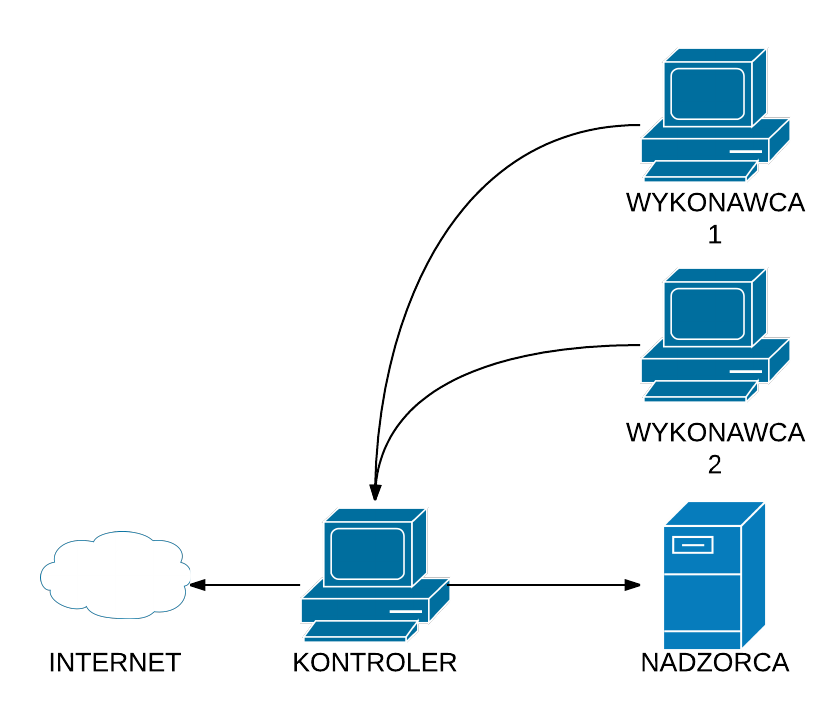
\includegraphics[scale=1.0]{gfx/schema-network.png}
		\caption{Schemat połączeń sieciowych}
		\label{gfx-schema-network}
	\end{figure}
	
	Jedyną maszyną systemu wymagającą bezpośredniego dostępu do Internetu jest Kontroler. Jest on połączony odrębnymi połączeniami sieciowymi również z Nadzorcą oraz Wykonawcami. Za pośrednictwem Kontrolera dostęp do sieci Internet mają również Wykonawcy. Ich dostęp jednakże jest ograniczony poprzez zaporę uruchomioną na Kontrolerze: nie mają oni dostępu do sieci lokalnych (adresy lokalne: 192.0.0.1/8 i~adresy zawierające pulę Politechniki: 194.0.0.0/8), nie mogą również nawiązywać nowych połączeń z maszyną Kontrolera. Również na Kontrolerze użytkownik systemu może podejrzeć ruch sieciowy wykonawców (np. za pomocą polecenia \textit{tcpdump}).
	
	Poniżej znajduje się opis i adresy sieci działających w ramach MESS. Adresy IP poszczególnych maszyn środowiska znajdują się w tabeli \ref{tab-network}.
	
	\subsubsection{Kontroler - Internet}
	
	Konfiguracja MESS zakłada, że połączenie Kontrolera z siecią Internet jest realizowane za pomocą interfejsu sieciowego \textit{eth0}. Pozostałe parametry (tj. adres IP, wykorzystanie bądź nie DHCP, etc.) nie ma wpływu na działanie środowiska.
	
	\subsubsection{Kontroler - Nadzorca}
	
	Kontroler i Nadzorca komunikują się w~ramach sieci 192.168.141.0/24. Do tejże sieci nie powinny mieć dostępu żadne inne maszyny.
	
	\subsubsection{Kontroler - Wykonawca}
	
	Wykonawcy komunikują się z~Kontrolerem (oraz efektywnie - z~siecią Internet) za pośrednictwem sieci 192.168.151.0/24. Podobnie jak w przypadku sieci \textit{Kontroler-Nadzorca}, żadne inne maszyny nie powinny mieć dostępu do tejże sieci.
	
	\begin{table}
		\begin{tabular}[th]{|c|c|c|c|c|}
			\hline & Adres IP & Adres IP  & Adres IP & Adres IP \\
			Sieć & Kontrolera & Nadzorcy & Wyk. 1 & Wyk. 2 \\
			\hline 192.168.141.0/24 & 192.168.141.2 & 192.168.141.1 & - & - \\
			\hline 192.168.151.0/24 & 192.168.151.2 & - & 192.168.151.11 & 192.168.151.12 \\
			\hline		
		\end{tabular}
		\label{tab-network}
		\caption{Adresy maszyn MESS w sieciach wewnętrznych środowiska}
	\end{table}	
	
	\subsection{Kontroler}
	
	\subsubsection{Moduł serwera MESS}
	
	Moduł serwera MESS jest głównym modułem aplikacji. Jest on odpowiedzialny za komunikację z użytkownikiem oraz wydawanie odpowiednich poleceń Nadzorcy oraz Wykonawcom. Ponadto, na Kontrolerze przechowywane są wyniki kilku ostatnich eksperymentów wykonywanych w środowisku. Moduł został napisany w języku Python \cite{www-python} i składa się z następujących części:
	\begin{itemize}
		\item \textit{WorkerAPI}, które odpowiada za komunikację z~modułami aplikacji Wykonawcy. Do zadań WorkerAPI należy przechowywanie aktualnego stanu Wykonawcy, wysyłanie do niego komunikatów oraz pobieranie i~zapisywanie plików z~wynikami w lokalizacji widzianej przez serwer HTTP.
		
		Aktualny stan każdego Wykonawcy jest przechowywany w~celu weryfikacji żądań przychodzących od klienta. Dzięki niemu środowisko nie dopuszcza do uruchomienia eksperymentu na maszynie będącej w~użyciu bądź próby pobrania wyników z~wyłączonego Wykonawcy.
		
		\item \textit{SupervisorAPI}, które komunikuje się z~Nadzorcą. Jest ono odpowiedzialne za wysyłanie żądań do Nadzorcy platformy wirtualizacji i~oczekiwanie na ich ukończenie.
		
		Ponieważ przetwarzanie żądania startu, zatrzymania bądź przywrócenia stanu maszyny wirtualnej jest czasochłonne, oczekiwanie na odpowiedź w~ramach jednego żądania HTML mogłoby doprowadzić do błędu przekroczenia czasu na odpowiedź. Z tego powodu po wysłaniu żądania zmiany stanu maszyny wirtualnej \textit{WorkerAPI} odpytuje cyklicznie Nadzorcę o~stan danej maszyny do momentu, kiedy ta znajdzie się w stanie nieprzejściowym.
		
		\item \textit{RPCService}, które jest usługą XMLRPC przeznaczoną do użytku przez użytkowników środowiska. Udostępnia ona następujące metody:
		\begin{itemize}
			\item \textit{get\_vm\_state} 
			
			Odpytuje \textit{WorkerAPI} o~aktualny stan żądanego Wykonawcy i~zwraca wynik (\textit{Wolny}, \textit{Pracuje}).
			
			\item \textit{purge\_result\_files} 			
			
			Usuwa pliki z wynikami eksperymentów przeprowadzonych na podanym Wykonawcy oprócz podanej liczby najświeższych wyników.
			
			\item \textit{restart\_vm}
			
			Wykonuje restart podanego Wykonawcy. W~tym celu wywołuje odpowiednią metodę \textit{WorkerAPI}, która przesyła żądanie dalej do aplikacji danego Wykonawcy.
			
			\item \textit{start\_analysis}
			
			Rozpoczyna eksperyment na podanym Wykonawcy. W~tym celu za pośrednictwem \textit{SupervisorAPI} żąda przywrócenia stanu maszyny Wykonawcy i uruchomienia go. Następnie przesyła otrzymane dane próbki i~zestawu narzędzi użytkownika do aplikacji Wykonawcy za~pośrednictwem \textit{WorkerAPI}.
			
			\item \textit{stop\_analysis}
			
			Metoda domyślnie kończy eksperyment na podanym Wykonawcy i~zwraca nazwę utworzonego pliku wynikowego. W~tym celu za pośrednictwem \textit{WorkerAPI} żąda od Wykonawcy zatrzymania eksperymentu, Następnie, również za pomocą modułu \textit{WorkerAPI}, ściąga wyniki do katalogu widocznego przez serwer HTTP. Po pobraniu pliku maszyna Wykonawcy jest wyłączana za pośrednictwem \textit{SupervisorAPI}, a~jako wynik metody zwracana jest nazwa pobranego pliku wyników.
			
			Metoda \textit{stop\_analysis} wywołana z~parametrem \textit{force} nie wykonuje początkowych kroków (tj. pobierania wyników), ale jedynie sprowadza maszynę wirtualną Wykonawcy do stanu wyłączonego. Jest ona przeznaczona do obsługi sytuacji, kiedy użytkownik nie jest już zainteresowany wynikami eksperymentu, bądź też zakończenie eksperymentu ze ściągnięciem tychże wyników jest niemożliwe.
						
		\end{itemize}
	\end{itemize}
	
	\subsubsection{Moduł zapory sieciowej / NAT}
	
	Maszyna Kontrolera odpowiada również za filtrowanie ruchu pomiędzy Wykonawcami a~siecią Internet. W tym celu program \textit{iptables} został skonfigurowany tak, aby zapewniał Wykonawcom dostęp do Internetu poprzez NAT. Jednocześnie razem z translacją w regułach \textit{iptables} zdefiniowane jest filtrowanie pakietów - wycięty jest ruch z Wykonawców na adresy sieci lokalnej lub zdefiniowane porty.
	
	\subsubsection{Serwer HTTP}
		
	Na maszynie Kontrolera uruchomiony jest serwer HTTP, za pośrednictwem którego użytkownik ma możliwość pobrania archiwum z wynikami eksperymentu. Powodem takiego rozwiązania jest zaobserwowany podczas testów środowiska problem -  przesyłanie wyników za pomocą protokołu XMLRPC w dużej części kończyło się niepowodzeniem ze względu na zbyt duży rozmiar pliku. Z~tego powodu pobieranie wyniku odbywa się osobnym kanałem.

	\subsubsection{Konfiguracja Kontrolera}
	
	Kontroler podczas startu odczytuje plik konfiguracyjny \textit{mess-config.ini}. Plik ten zawiera konfigurację nasłuchu usługi XMLRPC, adresy i~porty aplikacji Wykonawców oraz Nadzorcy, katalog i maksymalną liczbę plików wynikowych. Struktura pliku konfiguracyjnego dla środowiska z~dwoma Wykonawcami wygląda następująco:
\begin{lstlisting}
[Controller]
listen_address =
listen_port = 2811
supervisors = HyperV1
results_dir = /home/analysis/results/
results_cache_size = 10
workers = MW1,MW2

[HyperV1]
ip = 192.168.141.1
port = 8989

[MW1]
ip = 192.168.151.11
port = 5501

[MW2]
ip = 192.168.151.12
port = 5501
\end{lstlisting}

	\subsection{Nadzorca}	
	
	\subsubsection{Moduł serwera Nadzorcy}
	Na maszynie Nadzorcy znajduje się tylko jeden moduł MESS i jest on odpowiedzialny za sterowanie maszynami wirtualnymi. Udostępnia on Kontrolerowi za pomocą protokołu HTTP proste API pozwalające na sterowanie maszynami wirtualnymi. API ma postać:
	\begin{itemize}
		\item \textit{vmName/status}
		
		Zwraca obecny stan maszyny \textit{vmName}. Z punktu widzenia MESS naistotniejszymi kodami odpowiedzi są:
		\begin{itemize}
			\item \textit{Running}: maszyna jest uruchomiona (działa),
			\item \textit{Off}: maszyna jest wyłączona i~nie jest załadowana żadna migawka,
			\item \textit{Saved}: maszyna nie wyłączony, ale ma zapisany stan (została uśpiona bądź została wczytana migawka).
		\end{itemize}
	
		\item \textit{vmName/start}
		
		Uruchamia maszynę wirtualną o~nazwie \textit{vmName}.
		
		\item \textit{vmName/stop}
		
		Zatrzymuje maszynę wirtualną \textit{vmName}.
	
		\item \textit{vmName/snapshot/snapshotName/apply}
		
		Przywraca maszynę wirtualną \textit{vmName} do stanu migawki o~nazwie \textit{snapshotName}.
	\end{itemize}
	
	Moduł został zaimplementowany w języku C\#. Wykorzystuje on WMI \cite{www-wmi} API (\textit{Windows Management Instrumentation}) do komunikacji z systemem Hyper-V, natomiast odbieranie komunikatów od Kontrolera jest obsługiwane przez usługę WCF (ang. \textit{Windows Communication Foundation}). Sam moduł został podzielony na trzy klasy:
	\begin{itemize}
		\item \textit{HyperVService}, która zawiera interfejs i implementację usługi udostępnionej poprzez WCF \cite{www-wcf}. Wszystkie żądania są obsługiwane z wykorzystaniem pomocniczej metody \textit{ProcessRequest}. Jej zadaniem jest sprawdzenie poprawności wejściowego parametru \textit{vmName} (tj. nazwy maszyny wirtualnej, do której odnosi się żądanie), obsługa błędów przetwarzania żądania oraz odpowiednie sformatowanie wyjścia:
		\begin{lstlisting}[language={[Sharp]C}]
private Stream ProcessRequest(
  Func<String> requestHandler, String vmName) 
{
  if (!vmNameRegex.IsMatch(vmName)) {
    logger.Info("Illegal vmName: " + vmName);
   	return RespondAsText("ILLEGAL_VM_NAME");
  }

  try {
    String result = requestHandler();
    logger.Info("RequestHandler result: " + result);
    return RespondAsText(result);
  } catch(Exception exception) { 
    logger.Warn("Failed to handle request: " 
		+ exception.ToString());
    return RespondAsText(exception.ToString());
  }
}
		\end{lstlisting}
		
		\begin{lstlisting}[language={[Sharp]C}]
private Stream RespondAsText(string input) {
  WebOperationContext
    .Current
	.OutgoingResponse
	.ContentType = "text/plain";
		
  byte[] rawInput = Encoding.UTF8.GetBytes(input);
  return new MemoryStream(rawInput);
}
		\end{lstlisting}
	
		\item \textit{VMManager}, która stanowi warstwę abstrakcji nad WMI. Celem jej utworzenia jest dostarczenie czytelnego interfejsu dla \textit{HyperVService} ukrywającego szczegóły implementacyjne (w tym interfejs \textit{WMI}). Klasa dostarcza następujące metody:
		\begin{lstlisting}[language={[Sharp]C}]
class VMManager {
    public OperationStatus ApplySnapshot(
    	string vmName, string snapshotName)
    { ... }

    public uint ChangeVMStatus(
    	string vmName, VmState targetState)
    { ... }
    
    public VMStatus GetVMStatus(
    	string vmName)
    { ... }
}\end{lstlisting}

		\item \textit{Program}, która uruchamia aplikację, tj. tworzy usługę WCF i~przełącza ją w tryb nasłuchiwania i obsługi żądań. W celu uniknięcia aktywnego oczekiwania (realizowanego poprzez np. \textit{while(true) \{\}}) które prowadzi do zużycia do 100\% czasu procesora, wykorzystany został obiekt klasy \textit{EventWaitHandle}. Zatrzymuje on wykonanie funkcji \textit{Main} na wywołaniu \textit{eventWaitHandle.WaitOne()} bez konsumowania czasu CPU.
		
		\begin{lstlisting}[language={[Sharp]C}]
static void Main(string[] args) {
    XmlConfigurator.Configure();

    using (ServiceHost serviceHost = new ServiceHost(
    	typeof(HyperVService))) 
    {                
        logger.Info("Starting REST service");
        serviceHost.Open();
        EventWaitHandle eventWaitHandle;        
        eventWaitHandle = new EventWaitHandle(
        	false, EventResetMode.AutoReset, 
        	Guid.NewGuid().ToString());        	
        eventWaitHandle.WaitOne();
    }    
}
		\end{lstlisting}
		
		Moduł serwera nadzorcy dostarczany jest w formie pakietu MSI, który razem z modułem instaluje niezbędne zależności (np. pakiet .NET Framework).
	\end{itemize}
		
	
	\subsection{Wykonawca}		
	
	Na maszynie Wykonawcy MESS uruchamiane są dwa moduły: usługa oraz aplikacja. Podział ten wynika z wymagania jak najwcześniejszego startu narzędzi monitorujących podczas restartu systemu. W tym celu wbudowane w~Wykonawcę narzędzia uruchamiane są podczas startu systemu (przed zalogowaniem użytkownika) przez usługę systemową. Taka usługa jednakże nie może być użyta do uruchamiania narzędzi użytkownika oraz próbek, gdyż te mogą wymagać dostępu do sesji użytkownika. Poza tym, uruchamiana próbka byłaby uruchamiana przez proces inny niż potomek \textit{explorer.exe}, co mogłoby mieć wpływ na jej działanie (a zatem również na powodzenie eksperymentu).
	
	Oprócz modułów MESS na maszynie Wykonawcy zainstalowany i uruchomiony jest działający na standardowym porcie (80) serwer HTTP. Jego zadaniem jest udostępnienie do ściągnięcia przez Kontroler pliku wyników eksperymentu.
	
	\subsubsection{Moduł usługi wykonawcy}
	
	Moduł usługi wykonawcy, odpowiedzialny za uruchamianie narzędzi, również został zaimplementowany w języku C\#. W systemie operacyjnym jest on uruchamiany jako usługa systemowa, razem ze startem systemu Windows. 
	
	Ze względu na możliwość zrestartowania maszyny Wykonawcy, Wykonawca musi wiedzieć, czy pracuje w trybie oczekiwania na eksperyment, czy eksperyment jest w~trakcie. Od tej informacji zależy zachowanie aplikacji Wykonawcy w~momencie jej uruchomienia (które następuje po zalogowaniu użytkownika do systemu). Informacja ta jest zapisywana w~rejestrze systemu Windows w kluczu \textit{HKEY\_LOCAL\_MACHINE/SOFTWARE/MESS}. Odczytywaniem tychże wartości z~rejestru zajmuje się usługa Wykonawcy, korzystając z dedykowanej ku temu celu klasy:
	
	\begin{lstlisting}[language={[Sharp]C}]
public class WindowsRegistryProvider {
    public String GetDir(String dirName)
    { ... }
    
    public bool IsAnalysisEnabled()
    { ... }

    public void SetAnalysisEnabled(bool isEnabled)
    { ... }
}
	\end{lstlisting}	
	
	Drugim istotnym elementem usługi Wykonawcy są dostawcy narzędzi monitorujących. Są oni odpowiedzialni za uruchamianie i zatrzymywanie narzędzi. Każdy dostawca musi dziedziczyć klasę \textit{ToolProvider}:
	\begin{lstlisting}[language={[Sharp]C}]
abstract class ToolProvider {
    protected EventLog AppEventLog;
    protected String ResultsDirectory;
    protected String ToolDirectory;
    
    public ToolProvider(EventLog appEventLog, 
	    String resultsDirectory, 
	    String toolDirectory)
    {
        ResultsDirectory = resultsDirectory;
        ToolDirectory = toolDirectory;
        AppEventLog = appEventLog;
    }

    abstract public void Start();

    abstract public void Stop();

    protected Process CreateProcess(
    	String executablePath, 
    	String workingDirectory, 
    	String arguments)
    {
        Process process = new Process();
        process.StartInfo.Arguments = arguments;
        process.StartInfo.FileName = executablePath;
        process.StartInfo.WorkingDirectory = workingDirectory;
        return process;
    }
}
	\end{lstlisting}
	
	Dla każdego z~dostawców należy zaimplementować poniższe dwie metody:
	\begin{itemize}
		\item Metoda \textit{Start} ma za zadanie uruchomić narzędzie monitorujące. Może w~tym celu (choć nie musi!) wykorzystać pomocniczą metodę \textit{CreateProcess} upraszczającą tworzenie obiektów klasy \textit{Process}. Klasa ta reprezentuje uruchomione bądź nie procesy systemu operacyjnego i~pozwala m.in. na uruchamianie i~zatrzymywanie tychże (z~oczekiwaniem na zamknięcie - synchroniczne, bądź bez - asynchroniczne). Przykładowo, poniższy kod uruchamia polecenie \textit{procmon} z~parametrem \textit{/Terminate} i~katalogiem roboczym \textit{C:} po czym czeka na jego zakończenie:

		\begin{lstlisting}[language={[Sharp]C}]
String procmonPath 
  = Path.Combine(ToolDirectory, "Procmon.exe");
Process terminateProcmonProcess 
  = CreateProcess(procmonPath, @"C:\", @"/Terminate");
terminateProcmonProcess.Start();
terminateProcmonProcess.WaitForExit();
		\end{lstlisting}		

		\item Metoda \textit{Stop}, której zadaniem jest zatrzymanie narzędzia monitorującego. Jest ona niezbędna, by aplikacja Wykonawcy mogła uzyskać dostęp do pliku logu. W~zależności od narzędzia wymagać może to wykonania polecenia systemowego (analogicznego do polecenia uruchamiającego narzędzie) lub wysłania do działającego narzędzia sygnału nakazującego zakończenie pracy. W~tym celu również wykorzystuje się obiekt klasy \textit{Process}:
		\begin{lstlisting}[language={[Sharp]C}]
SomeProcess  = CreateProcess(execPath, @"C:\", args);
SomeProcess.Start();
/* ... */		
SomeProcess.Kill();
		\end{lstlisting}		
		
	\end{itemize}
	
	W MESS wbudowane są dwa narzędzia: \textit{Process Monitor} (monitor procesów działających w systemie Windows) oraz \textit{Wireshark} (monitor ruchu sieciowego). Każdy z~nich posiada własną definicję dostawcy w~formie klasy dziedziczącej po \textit{ToolProvider}. 
	
	Metody \textit{Start} i \textit{Stop} dostawców są wykorzystywane, gdy aplikacja Wykonawcy przesyła usłudze Wykonawcy żądanie odpowiednio rozpoczęcia lub zatrzymania analizy.
	
	Oprócz wyżej wymienionych komponentów, usługa wykonawcy zawiera również serwer REST służący do komunikacji z~aplikacją Wykonawcy. Jego API składa się z~czterech ścieżek:
	
	\begin{itemize}
		\item \textit{analysis\symbol{92}disable}: ustawia zapisany tryb działania Wykonawcy jako "oczekiwanie", przez co po restarcie systemu Windows nie zostaną one ponownie uruchomione;
	
		\item \textit{analysis\symbol{92}start}: ustawia zapisany tryb działania Wykonawcy jako "w~trakcie analizy" (dzięki czemu po restarcie systemu operacyjnego Wykonawcy praca narzędzi monitorujących zostanie wznowiona) i~uruchamia zainstalowane narzędzia monitorujące;
		
		\item \textit{analysis\symbol{92}status}: zwraca aktualny tryb działania Wykonawcy ("oczekiwanie" lub "w trakcie analizy");
		
		\item \textit{analysis\symbol{92}stop}: zatrzymuje wszystkie narzędzia monitorujące
	\end{itemize}
	
	Podobnie jak w przypadku modułu serwera Nadzorcy, moduł usługi Wykonawcy dostarczany jest jako pakiet MSI. Poza dostarczaniem zależności instalator tworzy również odpowiednie klucze w rejestrze oraz instaluje usługę w~systemie i~konfiguruje ją (tj. przełącza w tryb uruchamiania automatycznego).
	
	\subsubsection{Moduł aplikacji Wykonawcy}
	
	Moduł aplikacji Wykonawcy jest odpowiedzialny za komunikację z Kontrolerem środowiska, ściąganie i uruchamianie próbki i towarzyszącemu jej pakietowi narzędzi użytkownika oraz komunikację z usługą Wykonawcy. Aplikacja została napisana w języku Python i jest uruchamiana razem z systemem Windows.
	
	Komunikacja aplikacji z Kontrolerem odbywa się za pomocą protokołu XMLRPC. Za jego pośrednictwem moduł udostępnia następujące metody:
	\begin{itemize}
		\item \textit{start\_analysis} - uruchamia eksperyment na Wykonawcy.
		
		Uruchomienie eksperymentu na maszynie Wykonawcy zaczyna się od zapisania na dysku plików: próbki oraz narzędzi użytkownika. Pliki te są przesyłane w~formie zserializowanej, obsługą serializacji zajmuje się pakiet \textit{xmlrpc} dostarczany przez język Python. 
		 
		Kolejnym krokiem jest rozpakowanie zestawu i wywołanie skryptu \textit{before.ps1}, jeżeli takowy został dostarczony w archiwum. W~przeciwnym wypadku krok ten jest pomijany.
		 
		Następnie wysyłane jest do usługi Wykonawcy żądanie uruchomienia analizy, na które usługa włącza wbudowane narzędzia monitorujące. W~odpowiedzi aplikacja otrzymuje komunikat o pomyślnym uruchomieniu analizy lub o błędzie.
		 
		Jeżeli w trakcie przetwarzania wszystkich powyższych kroków nie wystąpił błąd, uruchamiana jest dostarczona próbka. Aplikacja nie czeka na zakończenie procesu próbki, ale od razu po utworzeniu procesu wysyła odpowiedź do Kontrolera o pomyślnym uruchomieniu eksperymentu. Jeżeli jednak błąd wystąpił, obsługę żądania kończy wysłanie Kontrolerowi odpowiedzi o błędzie uruchomienia próbki.
		
		\item \textit{restart} - wymusza restart systemu operacyjnego Wykonawcy.
		
		Restart wymaga wykonania trzech kroków. W pierwszym sprawdzane jest istnienie skryptu \textit{restart.ps1}. Jeżeli plik o takiej nazwie istnieje, jest on wykonywany.
		
		Następnie Aplikacja żąda od usługi Wykonawcy zatrzymania narzędzi monitorujących, a następnie wywołuje systemową komendę \textit{shutdown}:
		
		\begin{lstlisting}
shutdown /r /t 5
		\end{lstlisting}
		
		Po ponownym uruchomieniu systemu monitorowanie zostanie wznowione automatycznie.
		 
		\item \textit{stop\_analysis} - zatrzymuje narzędzia monitorujące i przygotowuje plik z wynikami.
		
		Pobieranie wyników zaczyna się analogicznie do restartu - żądaniem zatrzymania narzędzi monitorujących przez usługę Wykonawcy. Jednakże w~przeciwieństwie do restartowania maszyny, przy zatrzymywaniu eksperymentu usługa jest powiadamiana by nie uruchamiać narzędzi przy następnym uruchomieniu systemu.
		
		Następnie wywoływany jest skrypt \textit{after.ps1}. Analogicznie do pozostałych skryptów, krok ten jest pomijany jeżeli plik o~podanej nazwie nie istnieje.
		
		W kolejnym kroku tworzone jest archiwum ZIP zawierające wyniki działania narzędzi i skryptów. Plik ten jest umieszczany w lokalizacji widzianej przez uruchomiony na Wykonawcy serwer HTTP. 
	\end{itemize}
	
	\subsubsection{Serwer HTTP}
	Na maszynie Wykonawcy uruchomiony jest serwer HTTP, za pośrednictwem którego Kontroler pobiera wyniki eksperymentu. Podobnie jak w~przypadku Kontrolera, przesyłanie wyników za pomocą protokołu XMLRPC w~dużej części kończyło się niepowodzeniem ze względu na zbyt duży rozmiar pliku.
			 			 
	\subsection{Skrypty klienta}
	Razem ze środowiskiem stworzone zostały skrypty w języku Python pozwalające na wykonanie poniższych operacji:
	\begin{itemize}
		\item \textit{mess-start-analysis.py}: rozpoczyna eksperyment na zadanej maszynie Wykonawcy;
		\item \textit{mess-stop-analysis.py}: kończy eksperyment i pobiera wyniki z zadanej maszyny;
		\item \textit{mess-get-state.py}: zwraca stan maszyny Wykonawcy (Zajęty / Wolny),
		\item \textit{mess-purge-results.py}: usuwa pliki wynikowane eksperymentów wykonanych na zadanym Wykonawcy z Kontrolera, pozostawiając zadaną liczbę ostatnich wyników.
	\end{itemize}
	
	Skrypty dysponują wbudowaną pomocą objaśniającą niezbędne i opcjonalne parametry. Przykładowo pomoc dla polecenia \textit{mess-start-analysis} wygląda następująco:
	
	{\tiny 
	\begin{lstlisting}
~/MESS/Client $ ./mess-start-analysis.py   
Starts sample analysis on the VH worker VM.
Parameters:
-s --sample-file-path path/to/sample        REQUIRED    sample file to upload and analyse
-n --sample-target-name file.exe            REQUIRED    name for sample file on VM worker machine
-t --toolkit-file-path path/to/toolkit.zip  REQUIRED    additional toolkit file
-m --vm-name MW1                            REQUIRED    name of worker VM
		
	\end{lstlisting}
	}
	
	Wszystkie pliki skryptów klienckich wykorzystują sekcję \textit{[Client]} pliku konfiguracyjnego \textit{mess-config.ini}. Są z niej odczytywane dane adresu serwera Kontrolera MESS. Plik ma następującą strukturę:
	
	\begin{lstlisting}
[Client]
proxy_url = http://194.29.168.208:2811
results_url = http://194.29.168.208	
	\end{lstlisting}

	Oba parametry pliku konfiguracyjnego wskazują na położenie w sieci maszyny Kontrolera. Wartość \textit{proxy\_url} wskazuje na adres i port serwera XMLRPC, natomiast w \textit{results\_url} znajduje się adres, skąd klient może pobierać pliki wynikowe po zakończeniu eksperymentu.
	
	\clearpage
	\newpage	
			
	\section{Testy środowiska}
	
	W celu potwierdzenia przydatności środowiska zostały za jego pomocą wykonane eksperymenty złośliwego oprogramowania typu \textit{CryptoWall}. W~poniższym rozdziale został opisany jeden z~nich. System MESS został w~tym celu zainstalowany na jednej ze stacji roboczych Zakładu Oprogramowania i~Architektury Komputerów Instytutu Informatyki w~konfiguracji jak na rysunku~\ref{gfx--schema-basic-logical}. Wykonano z~jego wykorzystaniem szereg eksperymentów z~różnymi próbkami CryptoWall, zbierając dane o~łącznej wielkości ponad ... GiB.
	
	\subsection{Analizowana próbka}
	CryptoWall należy do oprogramowania typu \textit{ransomware}, tj. oprogramowania mającego na celu wyłudzić od ofiary korzyść materialną (najczęściej w~postaci okupu w~walucie \textit{Bitcoin}). W tym celu szyfruje dysk twardy ofiary szyfrem niesymetrycznym, a następnie wyświetla planszę analogiczną do przedstawionej na rysunku \ref{gfx-cryptowall-message}. 
	
	\begin{figure}[ht]
		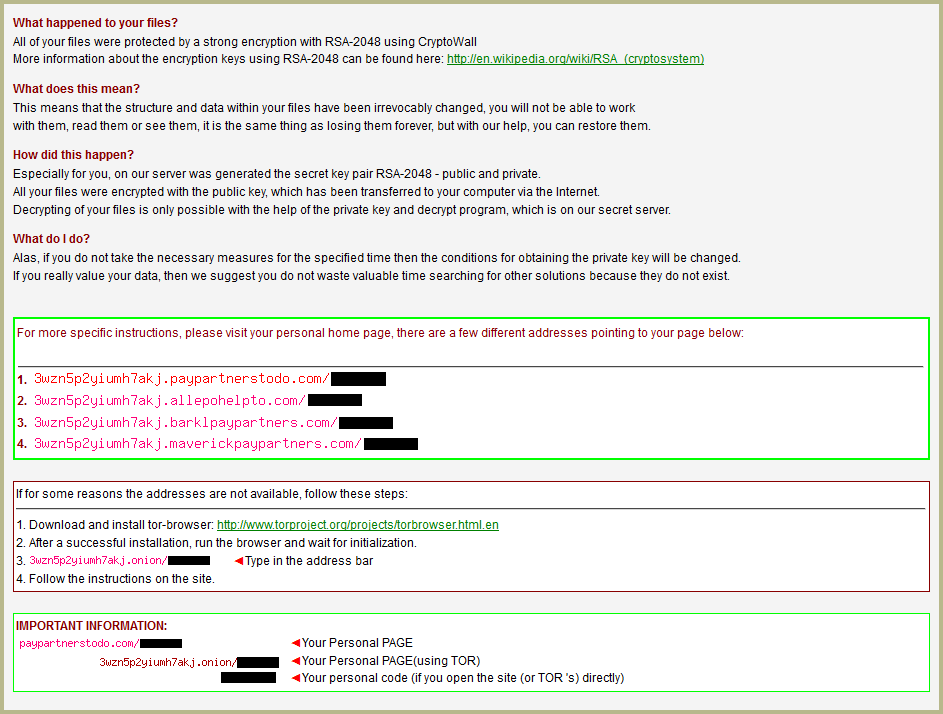
\includegraphics[scale=0.42]{gfx/cryptowall-message.png}
		\caption{Plansza wyświetlana przez \textit{CryptoWall}}
		\label{gfx-cryptowall-message}
	\end{figure}
	
	\subsection{Wyniki eksperymentu}
	
	Po przeprowadzeniu piętnastominutowego eksperymentu w~systemie MESS pobrane zostało archiwum z plikami wynikowymi. Zawierało ono plik dziennika programu Procmon oraz zrzut ruchu sieciowego wygenerowany przez Wireshark.
	
	\begin{figure}[ht]
		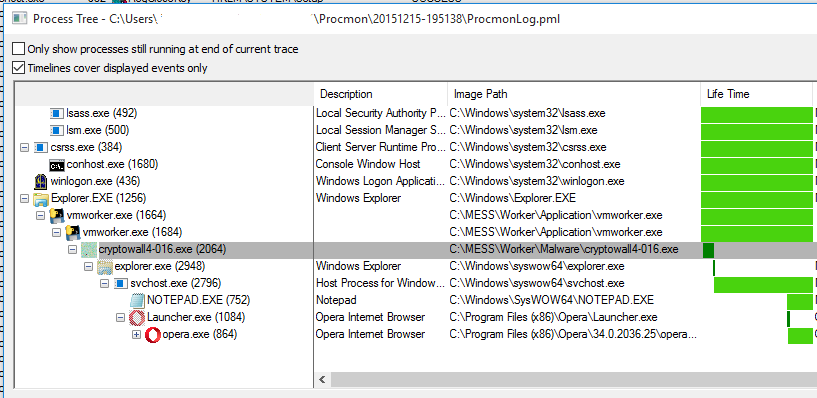
\includegraphics[scale=0.66]{gfx/anal-1-ptree.PNG}
		\caption{Drzewo procesów uruchomionych na maszynie Wykonawcy.}
		\label{gfx-anal-1-ptree}
	\end{figure}
	
	Plik logu monitora procesów (\textit{Procmona}) otworzony w~widoku drzewa procesów (p. Rysunek \ref{gfx-anal-1-ptree}) stanowi dobry punkt wyjścia do rozpoczęcia analizy wyników. Widoczne jest są nim informacje takie, jak czas trwania procesu próbki (tutaj: \textit{cryptowall4-016.exe}), jak i utworzonych przez nią procesów potomnych (\textit{explorer.exe} i~\textit{svchost.exe}; te ostatnie mają ścieżkę pliku .exe inną niż pliki uruchomione przez system Windows, dzięki czemu łatwa była ich identyfikacja w~pliku logu).

	\begin{figure}[ht]
		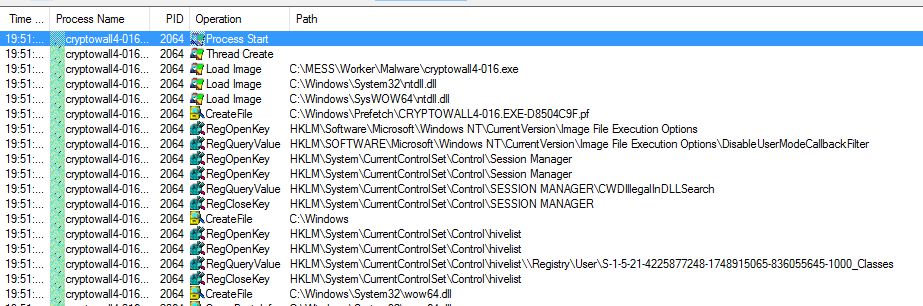
\includegraphics[scale=0.59]{gfx/anal-2-start.PNG}
		\caption{Rozpoczęcie działania procesu badanej próbki.}
		\label{gfx-anal-2-start}
	\end{figure}
	
	Z dziennika monitora odczytać można również kolejne zarejestrowane operacje wykonywane przez proces próbki. Rysunek \ref{gfx-anal-2-start} przedstawia moment uruchomienia \textit{Cryptowalla} (utworzenie procesu, załadowanie bibliotek DLL). Następnie próbka uruchomiła systemową aplikację \textit{explorer.exe}, po czym - za jej pomocą - wywołała narzędzie \textit{vssadmin.exe}, by usunąć kopie plików wykonane przez wbudowany w~system Windows mechanizm \textit{Volume Shadow Copy}. Następnie uruchomiona została aplikacja \textit{svchost.exe}, a próbka~przeszła do realizacji swojego podstawowego celu. Obserwowany program dokonywał zapisu w~znalezionych plikach użytkowników, a następnie tworzył w~zawierających je katalogach obrazek z~planszą analogiczną do rysunku \ref{gfx-cryptowall-message}.
	
	\begin{figure}[ht]
		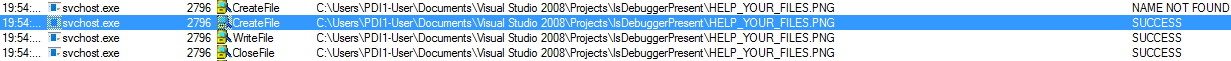
\includegraphics[scale=0.44]{gfx/anal-3-helpfiles.PNG}
		\caption{Działania wykonywane przez próbkę - tutaj: tworzenie plików z~planszą.}
		\label{gfx-anal-3-scamimg}
	\end{figure}	
	
	Choć program \textit{Procmon} oferuje bardzo bogate możliwości filtrowania danych -- w~tym również w czasie zbierania informacji do pliku -- filtrowanie danych przed ich zebraniem z~Wykonawcy nie jest zalecane. Jak widać na rysunku \ref{gfx-anal-3-scamimg}, niektóre działania próbki są prowadzone przez proces aplikacji wbudowanej w~sytem operacyjny (np. widoczny na rysunku \textit{svchost.exe} tworzący pliki z~planszami). Z~tego powodu zaleca się wykonywać operacje stratne dopiero po pobraniu rezultatów eksperymentu.
	
	\begin{figure}[ht]
		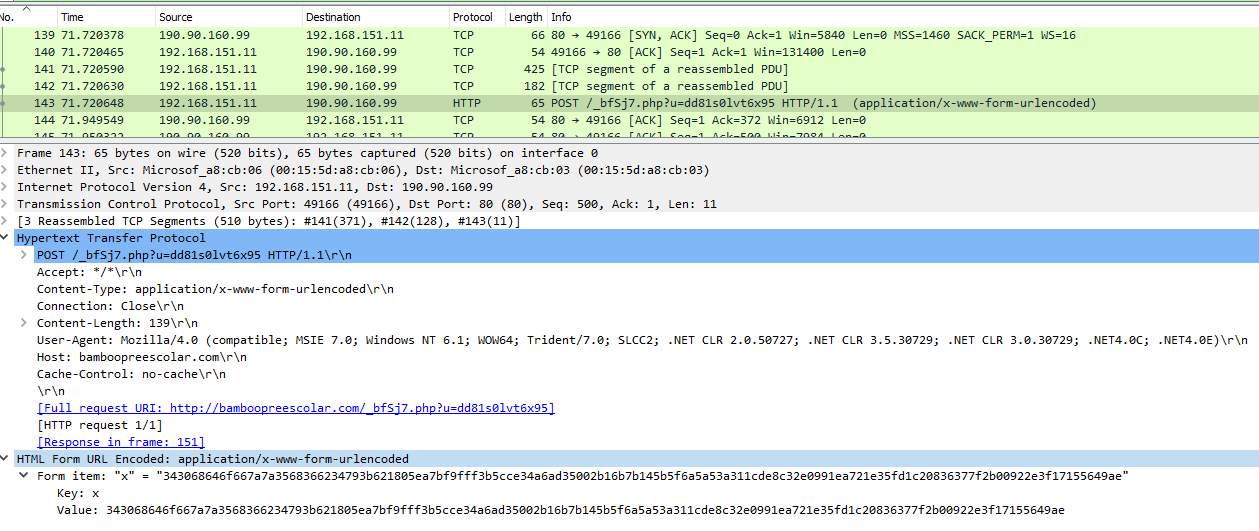
\includegraphics[scale=0.44]{gfx/anal-4-wireshark.PNG}
		\caption{Podgląd ruchu sieciowego - jedno z żądań wykonanych przez próbkę.}
		\label{gfx-anal-4-wireshark}
	\end{figure}	
	
	Archiwum wynikowe otrzymane na podstawie opisywanego eksperymentu zawiera również plik zrzutu sieciowego wykonanego programem \textit{Wireshark}. W~przypadku badanej próbki ruch pomiędzy komputerem Wykonawcy a~serwerem, z~którym się on łączył, był w dużej części zaszyfrowany. Rysunek~\ref{gfx-anal-4-wireshark} pokazuje wycinek ruchu - żądanie HTTP POST wysłane przez próbkę do zainfekowanego serwera służącego prawdopodobnie jako pośrednik pomiędzy maszynami ofiar a~serwerem sterującym\footnote{Dokładny opis infrastruktury \textit{CryptoWalla} oraz analiza jego zachowania w sieci są dostępne w~\cite{cryptowall-analysis}}.
	
	\clearpage
	\newpage
	
	\section{Podsumowanie}
	
	Wykonane eksperymenty potwierdziły użyteczność systemu MESS w~procesie analizy złośliwego oprogramowania. Choć jeszcze przed uruchomieniem eksperymentu znany był sposób ogólny działania próbki i~jej zachowanie w~sieci, zebrane pliki dostarczyły informacji o~operacjach wykonywanych na systemie operacyjnym i~jego składnikach. 
	
	Jednocześnie w~wyniku przeprowadzonych eksperymentów zidentyfikowane zostały obszary, w~których środowisko należałoby usprawnić bądź rozbudować. Do potencjalnych kierunków rozwoju systemu należą: automatyczna wstępna analiza zebranych danych oraz rozwój aplikacji stanowiącej repozytorium próbek do~analizy lub integracja z~innymi systemami (np. z~wykorzystywanymi w~Instytucie Informatyki PW systemami HoneyPot i~analitycznymi \cite{qnap-malware, honeypots}).
		
	Ze względu na dużą ilość danych z~punktu widzenia użytkownika korzystne byłoby prezentowanie bezpośrednio po zakończeniu eksperymentu informacji takich jak:
	
	\begin{itemize}
		\item czas działania procesu próbki i~jego procesów potomnych,
		\item adresy maszyn z którymi łączono się z maszyny Wykonawcy.
	\end{itemize} 
	
	Powyższe informacje pozwoliłyby użytkownikowi szybko ocenić, czy eksperyment się powiódł (tj. czy próbka pomyślnie uruchomiła się na maszynie Wykonawcy i~nawiązała kontakt z~serwerem zarządzającym).
			
	Analogicznie do projektu Konsoli zarządzającej systemem Maltester, istotnym ułatwieniem pracy z MESS byłoby stworzenie aplikacji pośredniczącej pomiędzy użytkownikiem a~serwerem środowiska. Aplikacja ta mogłaby wspomóc użytkownika zapewniająć następujące funkcje:
	\begin{itemize}
		\item \textit{Przechowywanie próbek uruchomionych w~środowisku}
		
		MESS nie przechowuje w~żadnej formie uruchamianych próbek. Dodanie w~aplikacji pośredniczącej opcji przechowywania próbek przyspieszyłoby wykonywanie powtórnych eksperymentów.
		
		Potencjalnym rozszerzeniem tej funkcji jest automatyczne wykonywanie eksperymentów z~użyciem danej próbki. Użytkownik definiowałby czas trwania jednego eksperymentu, liczbę eksperymentów do~przeprowadzenia oraz migawki bądź maszyny wykorzystywane przy kolejnych eksperymentach. Funkcja ta pozwalałaby na np. określenie warunków, jakie musi spełnić system ofiary, by badana próbka pomyślnie uruchomiła się. Takimi warunkami może być obecność określonych aplikacji w~systemie i~ich wersja, konfiguracja samego systemu operacyjnego bądź obecność określonych jego aktualizacji.
		
		\item \textit{Prowadzenie eksperymentów o zaplanowanym czasie trwania}
		
		System MESS nie obsługuje innego zakańczania eksperymentu niż na żądanie użytkownika, ponieważ wiązałoby się m.in. to z~problemem dostarczenia wynikowego archiwum -- system nie jest zaprojektowany do przechowywania archiwalnych rezultatów. Niedogodność ta może zostać wyeliminowana przez aplikację przechowującą wyniki eksperymentów. Mogłaby ona również udostępniać funkcję tworzenia analiz planowanych, tj. trwających z~góry określony czas. Po upływie danego okresu od momentu uruchomienia aplikacja żądałaby zatrzymania eksperymentu, po czym sama pobierała wyniki i~zapisywała je we~własnej bazie.
	\end{itemize}
		
	Kolejnym kierunkiem rozwoju jest wykorzystanie innych platform wirtualizacji.
	Złośliwe oprogramowanie badane przy użyciu środowiska MESS często wyposażone jest w~mechanizmy wykrywania wirtualizacji. Dzięki nim program jest w~stanie stwierdzić, że działa na maszynie wirtualnej, a~następnie zatrzymać swoje działanie. Jednakże, ponieważ różne platformy wirtualizacji wymagają różnych mechanizmów ich wykrywania, również badane próbki mogą wykrywać jedne platformy, jednocześnie nie zauważając innych. Jednym ze sposobów zaadresowania tego problemu jest dywersyfikacja wykorzystywanych platform wirtualizacji. Na jedną z takich sytuacji napotkano podczas eksperymentów z~różnymi próbkami CryptoWalla -- jedna z~próbek skutecznie wykryła wirtualizację Xen systemu Maltester, nie zauważając wirtualizatora Hyper-V systemu MESS. Inna próbka natomiast skutecznie wykryła obecność wirtualizacji w~obu systemach.
	
	Ze względu na proste, wysokopoziomowe API wykorzystywane przez MESS do komunikacji z Nadzorcą maszyn wirtualnych, utworzenie modułu obsługującego platformy inne niż Hyper-V nie wymaga modyfikacji żadnego z~istniejących modułów. Konieczne jest jedynie utworzenie nowego modułu Nadzorcy oraz ewentualnie zmigrowanie istniejący maszyn wirtualnych z~formatu obecnego środowiska na nowy.		
	
	\clearpage
	\newpage	
	
	\section{Zawartość płyty CD}
	
	\clearpage
	\newpage
	
	\begin{thebibliography}{99}
	
	\bibitem{book-malware} Ed Skoundis, Lenny Zeltser \\
		{\it Malware. Fighting Malicious Code} \\
		Pearson Edication Inc. 2004
	
	\bibitem{cryptowall-analysis} Krzysztof Cabaj, Piotr Gawkowski, Konrad Grochowski, Dawid Osojca \\ {\it Network activity analysis of CryptoWall ransomware}\\
		Przegląd elektrotechniczny, nr 11/2015				
	
	\bibitem{qnap-malware} Krzysztof Cabaj, Konrad Grochowski, Piotr Gawkowski \\
		{\it Practical problems of Internet threats analyses} \\
		Springer-Verlag Berlin Heidelberg 2011
		
	\bibitem{honeypots} Krzysztof Cabaj, Piotr Gawkowski \\
		{it HoneyPot systems in practice} \\
		Przegląd elektrotechniczny, nr 2/2015
		
	\bibitem{weiti-maltester} Dawid Osojca \\ {\it Aplikacja wspierająca analizę złośliwego oprogramowania w~oparciu o monitor maszyn wirtualnym Xen } \\ Praca dyplomowa, Insystut Informatyki, Politechnika Warszawska 2012
	
	\bibitem{for-ultimate-antidbg} Peter Ferrie \\
		{\it The 'Ultimate' Anti - Debugging Reference} \\
		http://anti-reversing.com/Downloads/Anti-Reversing/The\_Ultimate\_Anti-Reversing\_Reference.pdf
	
	\bibitem{for-dynamic-anal} Ulrich Bayer, Andreas Moser, Christopher 
	Kruegel, Engin Kirda. \\
		{\it Dynamic analysis of malicious code} \\
		 Journal in Computer Virology, vol. 2, str. 67-77, 2006 
		 
	\bibitem{for-antivm-antidbg} Chen X., Andersen J., Mao Z.M., Bailey M., 
	Nazario J. \\
		{\it Towards an understanding of anti-virtualization 
			and anti-debugging behavior in modern malware} \\
		IEEE International Conference on Dependable Systems and 
		Networks, (2008), 177-186 

	\bibitem{www-malware-phases} The Four Phases of Every Attack \\
		https://blogs.mcafee.com/business/the-four-phases-of-every-attack/
	
	\bibitem{www-stuxnet} The Real Story of Stuxnet \\
		http://spectrum.ieee.org/telecom/security/the-real-story-of-stuxnet
	
	\bibitem{www-virus-winupdate} Symantec Security Response: \textit{W32.Downadup.B} 
		http://www.symantec.com/security\_response/writeup.jsp?docid=2008-123015-3826-99\&tabid=2
		
	\bibitem{www-classification} Kaspersky Lab - Malware Classifications \\
		http://www.kaspersky.com/internet-security-center/threats/malware-classifications
	
	\bibitem{www-niebezp-kaspersky} Wreszcie ktoś zrobił całkiem dobry fake-mail, czyli "twój bank i Kaspersky" chcą zainfekować twojego Androida \\
		https://niebezpiecznik.pl/post/wreszcie-ktos-zrobil-calkiem-dobry-fake-mail-czyli-twoj-bank-i-kaspersky/
	
	\bibitem{www-niebezp-fb} Wigilijny robak na Facebooku \\ 		
		https://niebezpiecznik.pl/post/wigilijny-robak-na-facebooku/
	
	\bibitem{www-anubis} Anubis - Malware Analysis for Unknown Binaries: \\
		http://anubis.iseclab.org/
		
	\bibitem{www-hpc} Capture-HPC Client Honeypot \\
		https://projects.honeynet.org/capture-hpc/
		
	\bibitem{tool-procmon} Process Monitor \\
		https://technet.microsoft.com/pl-pl/sysinternals/bb896645.aspx
		
	\bibitem{tool-wireshark} Wireshark \\
		https://www.wireshark.org/
		
	\bibitem{www-hyperv} Platforma Hyper-V \\
		https://www.microsoft.com/pl-pl/server-cloud/solutions/virtualization.aspx
	
	\bibitem{www-python} Python programming language \\
		https://www.python.org/
		
	\bibitem{www-wcf} Windows Communication Foundation \\
		https://msdn.microsoft.com/en-us/library/dd456779\%28v=vs.110\%29.aspx
					
	\bibitem{www-wmi} Windows Management Instrumentation \\
		https://msdn.microsoft.com/en-us/library/aa384642\%28v=vs.85\%29.aspx
					
	\end{thebibliography}	
	
	\clearpage
	\newpage	
	
	\section{Załącznik: instrukcja użytkownika}
	
	Niniejszy załącznik zawiera instrukcję instalacji i~użytkowania systemu MESS.
	
	\subsection{Instalacja i~przygotowanie i środowiska}
	
	\subsubsection{Konfiguracja Kontrolera}
	
	\subsubsection{Konfiguracja Nadzorcy}
	
	\subsubsection{Konfiguracja Wykonawcy}
	
	\subsection{Wykonywanie eksperymentów}
	
	\subsubsection{Przygotowanie}
	
	\subsubsection{Rozpoczęcie eksperymentu}

	\subsubsection{Restartowanie Wykonawcy}
	
	\subsubsection{Zatrzymanie eksperymentu}	

\end{document}